\documentclass[a4paper,12pt]{report}  % Document type, paper size, and font size

\usepackage[italian]{babel}  % Set language to italian

\usepackage[utf8]{inputenc}  % Character encoding
\usepackage[T1]{fontenc}
\usepackage{amsmath}         % Package for mathematics
\usepackage{amsfonts}        % Package for math fonts
\usepackage{amssymb}         % Package for math symbols
\usepackage{graphicx}        % Package for inserting images
\usepackage{geometry}        % Package to manage page margins
\usepackage{fontspec}        % Package for custom fonts
\usepackage{hyperref}        % Package for hyperlinks
\usepackage{xcolor}          % Package for colors
\usepackage{listings}        % Package for code listings
\usepackage{tcolorbox}
\usepackage{emoji}
\usepackage{multirow}
\usepackage{siunitx}
\usepackage{colortbl}
\usepackage{booktabs}
\usepackage{animate}

\geometry{top=2.5cm, bottom=2.5cm, left=2.5cm, right=2.5cm}  % Set page margins

\setlength{\parindent}{0pt}

\definecolor{headercolor}{RGB}{230, 230, 250}
\definecolor{rowcolor1}{RGB}{245, 245, 255}
\definecolor{rowcolor2}{RGB}{255, 255, 255}

% Definizione colori moderni
\definecolor{backcolour}{RGB}{248, 248, 248}     % Sfondo leggermente grigio
\definecolor{codegreen}{RGB}{72, 168, 96}        % Verde più soft per i commenti
\definecolor{codepurple}{RGB}{156, 39, 176}      % Viola più moderno
\definecolor{codered}{RGB}{219, 68, 55}          % Rosso Google-style
\definecolor{codeblue}{RGB}{66, 133, 244}        % Blu Google-style
\definecolor{codeorange}{RGB}{255, 111, 0}       % Arancione vivace
\definecolor{numbercolor}{RGB}{102, 102, 102}    % Grigio per i numeri di riga
\definecolor{definecolor}{RGB}{255, 128, 0}

\lstdefinestyle{mystyle}{
    backgroundcolor=\color{backcolour},
    commentstyle=\color{codegreen},
    keywordstyle=\color{codepurple},
    stringstyle=\color{codered},
    basicstyle=\fontspec{JetBrains Mono}\scriptsize,
    numberstyle=\fontspec{JetBrains Mono}\scriptsize\color{numbercolor},
    breakatwhitespace=false,
    breaklines=true,
    captionpos=b,
    keepspaces=true,
    numbers=left,
    numbersep=8pt,
    showspaces=false,
    showstringspaces=false,
    showtabs=true,
    tabsize=4,
    frame=single,
    rulecolor=\color{backcolour!70},
    xleftmargin=2.5em,
    framexleftmargin=2em,
    literate=
        {*}{{*}}1
        {\#}{{\textcolor{codepurple}{\#}}}1
}

\lstdefinestyle{bash}{
    backgroundcolor=\color{backcolour},
    commentstyle=\color{codegreen},
    keywordstyle=\color{codepurple},
    stringstyle=\color{codered},
    basicstyle=\fontspec{JetBrains Mono}\scriptsize,
    numberstyle=\fontspec{JetBrains Mono}\scriptsize\color{numbercolor},
    breakatwhitespace=false,
    breaklines=true,
    captionpos=b,
    keepspaces=true,
    numbers=left,
    numbersep=8pt,
    showspaces=false,
    showstringspaces=false,
    showtabs=true,
    tabsize=4,
    frame=single,
    rulecolor=\color{backcolour!70},
    xleftmargin=2.5em,
    framexleftmargin=2em,
    literate=
        {*}{{*}}1
}

% Apply the style
\lstset{style=mystyle}

% New command for inline code with background color
\newcommand{\lstinlinebg}[1]{\colorbox{backcolour}{\lstinline|#1|}}

% New command for inline code in italics with background color
\newcommand{\lstinlinebgit}[1]{\colorbox{backcolour}{\textit{\lstinline|#1|}}}

% New command for inline code in bold with background color
\newcommand{\lstinlinebgbf}[1]{\colorbox{backcolour}{\textbf{\lstinline|#1|}}}

% New command for inline code with big text
\newcommand{\lstinlinebig}[1]{\colorbox{backcolour}{\lstinline[basicstyle=\fontspec{JetBrains Mono}\normalsize]|#1|}}

% Set hyperlink color and background color for the table of contents
\hypersetup{
    colorlinks=true,           % Enable color links
    linkcolor=blue,            % Link color
    filecolor=magenta,         % Link to files color
    urlcolor=blue,             % URL color
    pdfcreator={LaTeX},        % PDF creator
    pdfproducer={LaTeX},       % PDF producer
}

\title{Progetto di Ingegneria di Internet e Web: Trasferimento file su UDP}            % Title of the document
\author{Antonio Bernardini e Flavio Caporilli} % Author's name
\date{}               % Date (optional)

\begin{document}

% First page with title, author, and date
\maketitle  

\newpage  % Start a new page for Table of Contents

% Second page with Table of Contents
\tableofcontents

\newpage

\chapter{Architettura del sistema e scelte progettuali}

In questo capitolo vengono descritte le scelte progettuali e l'architettura del sistema implementato, con particolare enfasi sul protocollo di comunicazione.

\section{Introduzione}
Lo scopo del progetto è progettare ed implementare un'applicazione client-server per il trasferimento di file in linguaggio C, utilizzando l'API dei socket di Berkeley.
L'applicazione dovrà impiegare il servizio di rete senza connessione, ossia il protocollo UDP (socket di tipo \lstinlinebg{SOCK_DGRAM}) per la trasmissione dei dati.
Il software deve permettere:
\begin{itemize}
    \item La connessione client-server senza autenticazione;
    \item La visualizzazione sul client dei file disponibili sul server tramite il comando \lstinlinebg{LIST};
    \item Il download di un file dal server tramite il comando \lstinlinebg{GET};
    \item L'upload di un file sul server tramite il comando \lstinlinebg{PUT};
    \item Il trasferimento di file in modo affidabile.
\end{itemize}
La comunicazione tra client e server deve avvenire tramite un opportuno protocollo.
Il protocollo di comunicazione deve prevedere lo scambio di due tipi di messaggi:
\begin{itemize}
    \item \textit{messaggi di comando}: vengono inviati dal client al server per richiedere delle diverse operazioni;
    \item \textit{messaggi di risposta}: vengono inviati dal server al client, in risposta ad un comando, con l'esito dell'operazione.
\end{itemize}

\subsection{Funzionalità del server \emoji{file-cabinet}}
Il server, di tipo concorrente, deve fornire le seguenti funzionalità:
\begin{itemize}
    \item L'invio del messaggio di risposta al comando \lstinlinebg{LIST} al client richiedente; il messaggio di risposta contiene la lista dei file, ovvero la lista dei nomi dei file disponibili per la condivisione;
    \item L'invio del messaggo di risposta al comando \lstinlinebg{GET} contenente il file richiesto, se presente, o un opportuno messaggio di errore;
    \item La ricezione di un messaggio \lstinlinebg{PUT} contenente il file da caricare sul server e l'invio di un messaggio di risposta con l'esito dell'operazione.
\end{itemize}

\subsection{Funzionalità del client \emoji{bust-in-silhouette}}
Il client, di tipo concorrente, deve fornire le seguenti funzionalità:
\begin{itemize}
    \item L'invio del messaggio \lstinlinebg{LIST} per richiedere la lista dei nomi dei file disponibili;
    \item L'invio del messaggio \lstinlinebg{GET} per ottenere un file;
    \item La ricezione di un file, richiesta tramite il messaggio di \lstinlinebg{GET}, o la gestione dell'eventuale errore;
    \item L'invio del messaggio \lstinlinebg{PUT} per effettuare l'upload di un file sul server e la ricezione del messaggio di risposta con l'esito dell'operazione.
\end{itemize}

\begin{figure}[h]
    \centering
    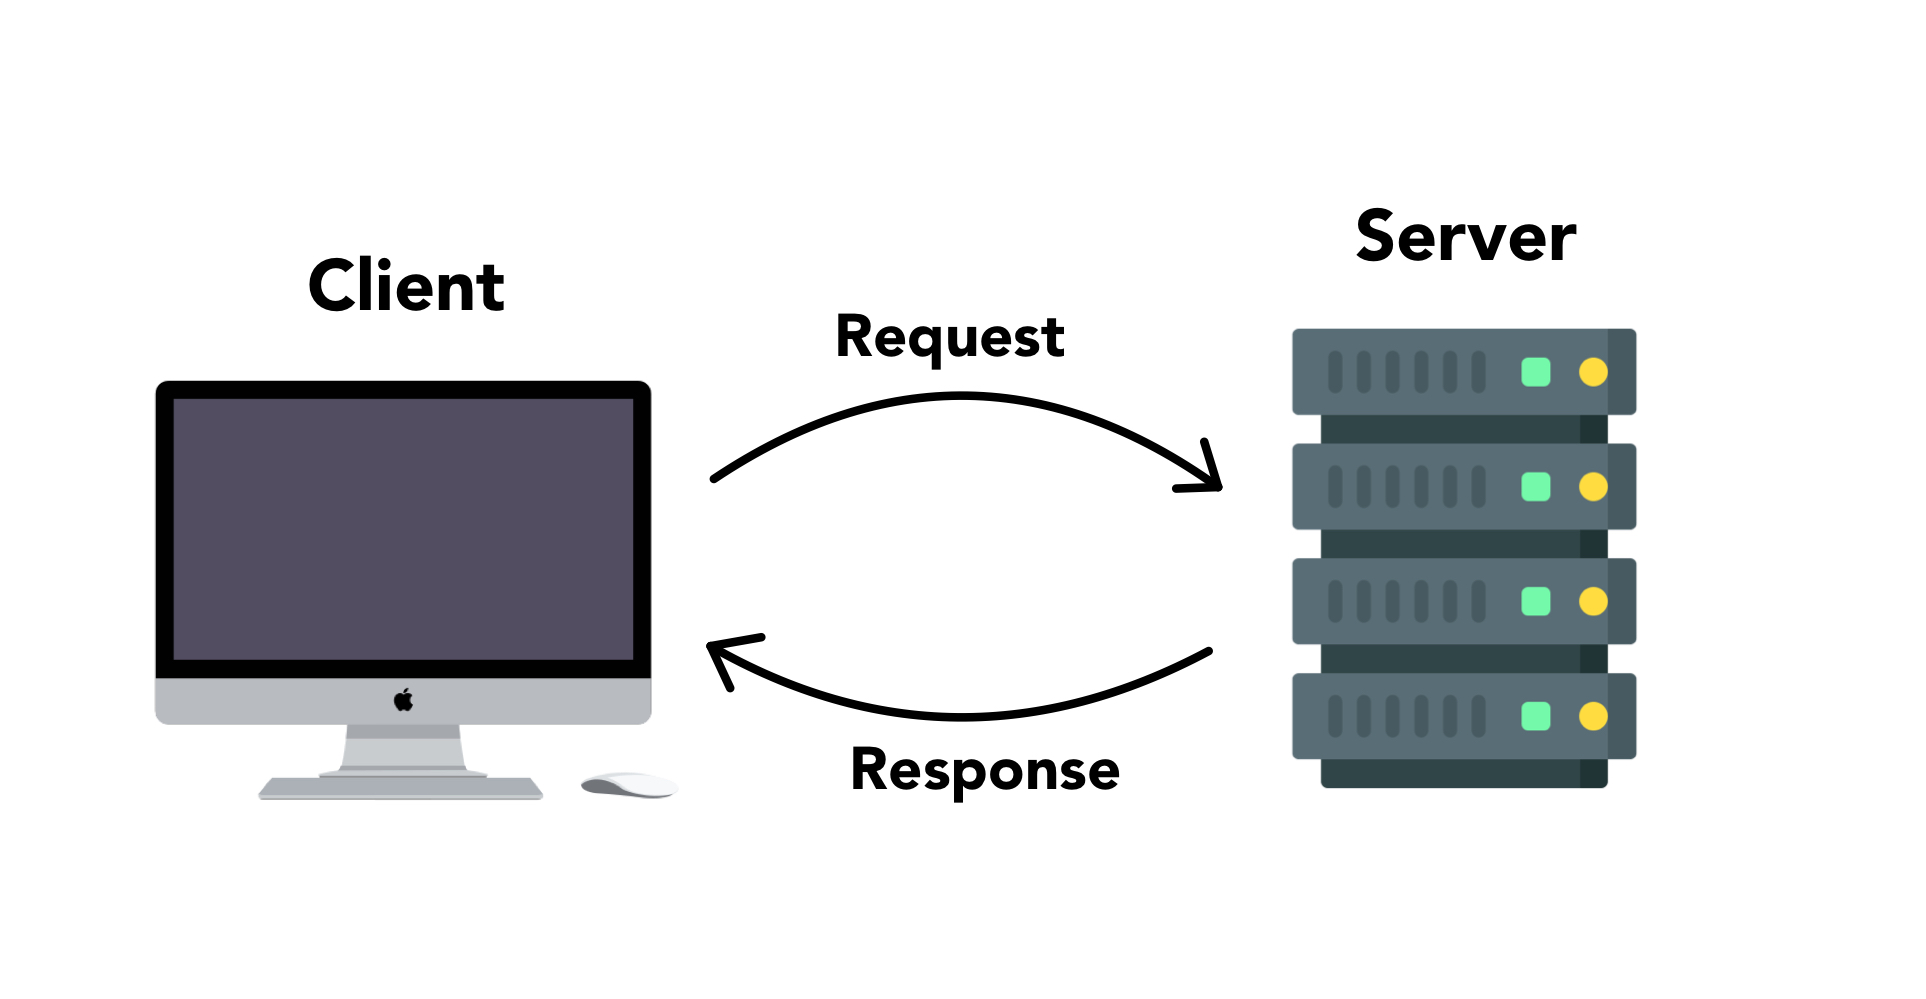
\includegraphics[width=0.6\textwidth]{imgs/01/client-server.jpeg}
    \caption{Schema client-server}
\end{figure}

\subsection{Trasmissione affidabile \emoji{handshake}}
Lo scambio di messaggi avviene usando un servizio di comunicazione non affidabile.
Al fine di garantire la corretta spedizione/ricezione dei messaggi e dei file sia i client che il server implementano a livello applicativo il protocollo \textit{Selective Repeat} con finestra di spedizione \lstinlinebg{WINDOW_SIZE}.
Per simulare la perdita dei messaggi in rete (evento alquanto improbabile in una rete locale per non parlare di quando client e server sono eseguiti sullo stesso host), si assume che ogni messaggio sia scartato dal mittente con probabilità \lstinlinebg{LOSS_PROBABILITY}.
La dimensione della finestra di spedizione \lstinlinebg{WINDOW_SIZE}, la probabilità di perdita dei messaggi \lstinlinebg{LOSS_PROBABILITY}, e la durata del timeout \lstinlinebg{TIMEOUT}, sono tre costanti configurabili ed uguali per tutti i processi.
Oltre all'uso di un timeout fisso (\textit{static timeout}), deve essere possibile scegliere l'uso di un valore per il timeout adattativo (\textit{adaptive timeout}) calcolato dinamicamente in base all'evoluzione dei ritardi di rete osservati.
I client ed il server devono essere eseguiti nello spazio utente senza richiedere privilegi di root.
Il server deve essere in ascolto su una porta di default (configurabile).

\section{Architettura del sistema \emoji{gear}}

\subsection{Organizzazione del progetto}
Il progetto S.P.Q.R. (\textit{Selective Protocol for Quality and Reliability}) consta di diverse directory\footnote{Si vuole specificare che la \textit{working directory} \lstinlinebg{spqr/} è composta fondamentalmente dalle directory citate.}, tra le più d'interesse troviamo:
\begin{itemize}
    \item \emoji{file-folder}\lstinlinebg{src/}: contiene i sorgenti del progetto, organizzato in file dedicati per lo sviluppo di specifiche funzionalità per il client e per il server;
    \item \emoji{file-folder}\lstinlinebg{include/}: contiene gli header del progetto, organizzati per modularità e riutilizzo del codice;
    \item \emoji{file-folder}\lstinlinebg{client-files/} e \emoji{file-folder}\lstinlinebg{server-files/}: nelle quali troviamo i file che il client e il server si scambiano tra loro;
    \item \emoji{file-folder}\lstinlinebg{tests/}: nella quale è presente lo script \lstinlinebg{integrity-consistency.py} che controlla l'integrità di ogni file inviato e/o ricevuto dal client e dal server;
    \item \emoji{file-folder}\lstinlinebg{tests/network/}: nella quale è presente lo script \lstinlinebg{list.pcapng} che riporta il traffico di rete generato dal client e dal server durante l'esecuzione del comando \lstinlinebg{LIST};
    \item \emoji{file-folder}\lstinlinebg{tests/performance/}: nella quale si trovano i grafici delle performance relativi al timeout statico, al timeout adattivo e alla comulazione degli errori;
    \item \emoji{file-folder} \lstinlinebg{docs/}: nella quale si trova il sito web del progetto.
\end{itemize}
Oltre alle directory citate, troviamo il \emoji{wrench}\lstinlinebg{Makefile} di particolare rilievo per automatizzare la compilazione del progetto.
Entrando più nel dettaglio, nella directory \lstinlinebg{src/} troviamo i seguenti file:
\begin{itemize}
    \item \emoji{page-facing-up}\lstinlinebg{client.c}: rappresenta il punto d'ingresso del client ed in particolare si occupa di gestire l'argomento \lstinlinebg{IPv4} (cioè l'indirizzo IP del server a cui i client devono connettersi) tramite riga di comando, istanzia il gestore dei segnali e tenta l'avvio della connesione con il server;
    \item \emoji{page-facing-up}\lstinlinebg{server.c}: rappreenta il punto d'ingresso del server, configura il socket principale, gestisce le connesioni in entrata e istanzia il gestore dei segnali;
    \item \emoji{page-facing-up}\lstinlinebg{common.c}: contiene funzioni e strutture condivise tra client e server (es: gestione timeout, progress bar, ASCII art, gestione degli errori, simulazione perdita pacchetti, ...);
    \item \emoji{page-facing-up}\lstinlinebg{protocol.c}: implementa il protocollo di trasferimento dati implementando il \textit{Selective Repeat} \emoji{incoming-envelope};
    \item \emoji{page-facing-up}\lstinlinebg{spqr_client.c}: implementa la logica del client, l'invio/ricezione pacchetti, comandi utente \lstinlinebg{LIST}, \lstinlinebg{GET}, \lstinlinebg{PUT} e gestione del comando aggiuntivo \lstinlinebg{CLOSE};
    \item \emoji{page-facing-up}\lstinlinebg{spqr_server.c}: implementa la logica del server, la gestione concorrente di client multipli e la bitmask per tracciare le connessioni attive.
\end{itemize}
Mentre, per quanto riguarda la directory \lstinlinebg{include/}, troviamo i seguenti file:
\begin{itemize}
    \item \emoji{page-facing-up}\lstinlinebg{stdc.h}: contiene tutte le librerie standard del linguaggio C e file header custom come \lstinlinebg{settings.h} e \lstinlinebg{common.h};
    \item \emoji{page-facing-up}\lstinlinebg{settings.h}: contiene le configurazioni globali e i parametri del progetto (es: il numero di porta, il numero massimo di client supportati, il timeout statico, il timeout adattivo, la dimensione della finestra, la probabilità di perdita, ...);
    \item \emoji{page-facing-up}\lstinlinebg{common.h}: contiene i prototipi delle funzioni e dei messaggi custom condivisi tra client e server;
    \item \emoji{page-facing-up}\lstinlinebg{protocol.h}: definizione delle strutture utili per il protocollo di trasferimento dati in modo affidabile implementanto tramite \textit{Selective Repeat} \emoji{incoming-envelope};
    \item \emoji{page-facing-up}\lstinlinebg{spqr_client.h}: prototipi della funzioni specifiche del client (es: gestione delle connesioni (\textit{Three-Way Handshake} con il server), gestione della terminazione con \lstinlinebg{ctrl+c}, ...);
    \item \emoji{page-facing-up}\lstinlinebg{spqr_server.h}: prototipi della funzioni specifiche del server (es: supporto a client multipli via \lstinlinebg{fork()}, risposta ai comandi \lstinlinebg{LIST}, \lstinlinebg{GET}, \lstinlinebg{PUT} e gestione del comando aggiuntivo \lstinlinebg{CLOSE}, ...).
\end{itemize}

\subsection{Protocollo Selective Repeat \emoji{incoming-envelope}}
L'architettura client-server progettata utilizza il protocollo di comunicazione non affidabile UDP per il trasferimento dei messaggi.
Tuttavia, per garantire l'affidabilità nella trasmissione dei file tra client e server, è stato implementato il protocollo \textit{Selective Repeat} \emoji{incoming-envelope}.
Questo protocollo ottimizza la gestione degli errori, riducendo al minimo le ritrasmissioni grazie alla selezione mirata dei pacchetti persi o corrotti, migliorando così l'efficienza complessiva del sistema.

\subsubsection{Funzionamento generale}
Il protocollo \textit{Selective Repeat} si basa sull'uso di una finestra scorrevole condivisa tra mittente e destinatario, consentendo l'invio e la ricezione di più pacchetti senza dover attendere una conferma immediata.
La dimensione della finestra determina il numero massimo di pacchetti che possono essere ``in volo" contemporaneamente.
Ogni pacchetto trasmesso è identificato da un numero di sequenza univoco, che permette al destinatario di riordinare correttamente i dati ricevuti.

A differenza di altri protocolli di affidabilità, il \textit{Selective Repeat} \emoji{incoming-envelope} utilizza ACK selettivi, ovvero conferme individuali per ogni pacchetto ricevuto, anche se fuori ordine.
I pacchetti non ancora riordinabili vengono temporaneamente memorizzati in un buffer, in attesa di ricevere quelli mancanti.

\subsubsection{Comportamento del Mittente}
Il mittente gestisce la trasmissione dei pacchetti rispettando la finestra di invio.
Ogni pacchetto viene inviato con un timer individuale che controlla il tempo massimo di attesa per la conferma.

Quando il mittente riceve un ACK, il pacchetto corrispondente viene marcato come confermato e la finestra scorre, consentendo l'invio di nuovi dati.
Se il timer di un pacchetto scade senza che sia stato ricevuto un ACK, il pacchetto viene ritrasmesso selettivamente, evitando di reinviare quelli già confermati.

\subsubsection{Comportamento del Destinatario}
Il destinatario, una volta ricevuti i pacchetti, segue una logica basata su bufferizzazione e riordinamento:
\begin{itemize}
    \item Accetta i pacchetti anche se ricevuti fuori ordine.
    \item I pacchetti non immediatamente utilizzabili vengono temporaneamente salvati in un buffer.
    \item Ogni pacchetto ricevuto genera un ACK, inviato al mittente indipendentemente dalla ricezione dei pacchetti precedenti.
    \item Se un pacchetto è già stato confermato in precedenza, eventuali ACK duplicati vengono ignorati dal mittente.
    \item Una volta ricevuti tutti i pacchetti fino a un certo numero di sequenza, i dati vengono consegnati all'applicazione in modo ordinato.
\end{itemize}

\begin{figure}[h]
    \centering
    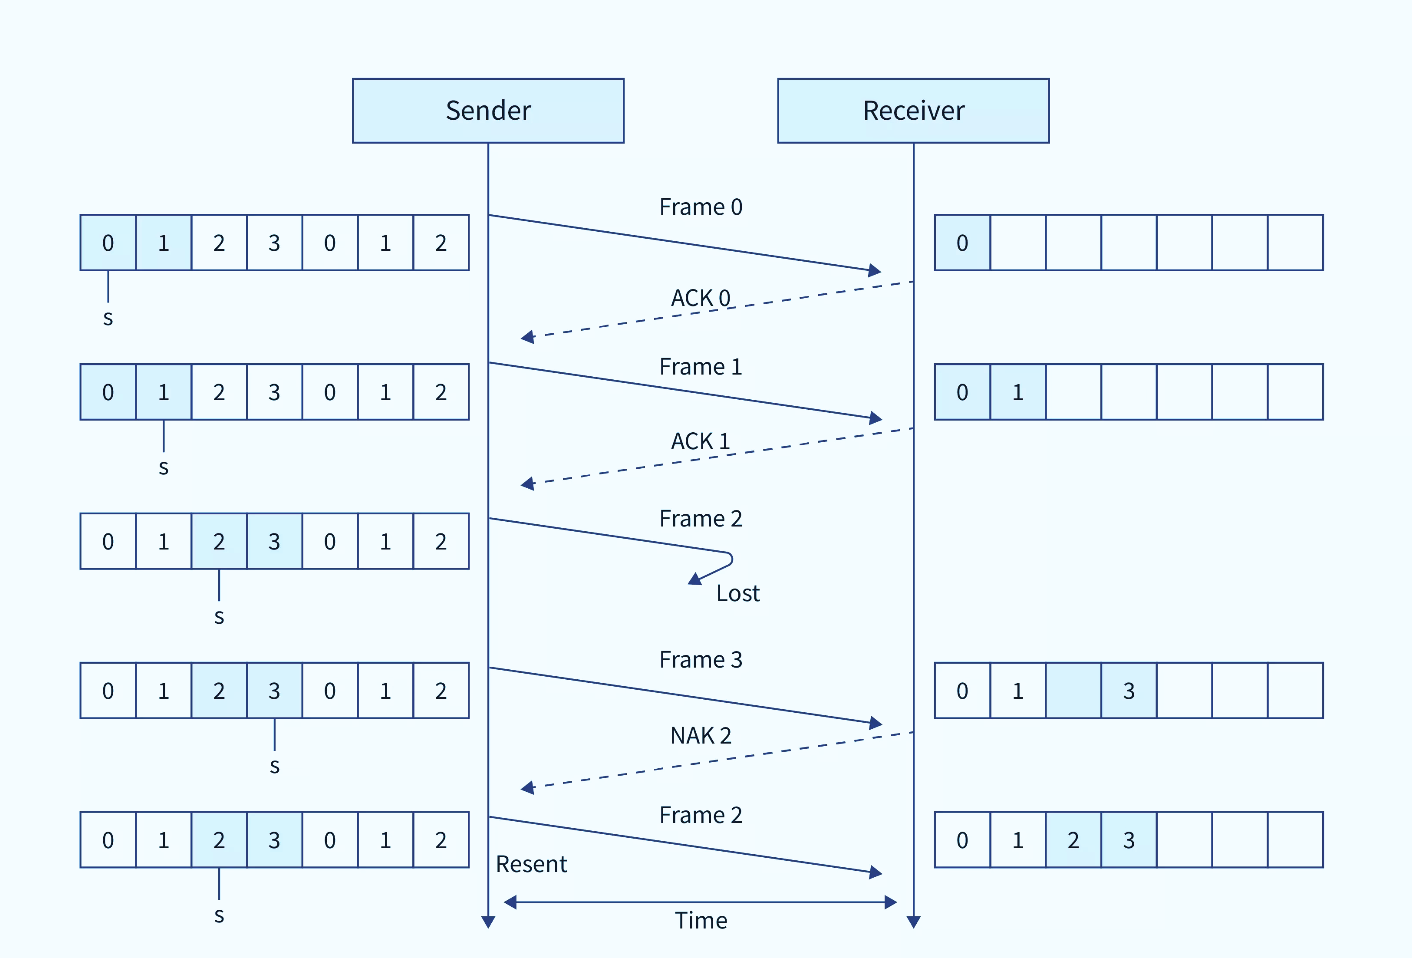
\includegraphics[width=0.75\textwidth]{imgs/01/sr.png}
    \caption{Funzionamento del protocollo \textit{Selective Repeat} \emoji{incoming-envelope}.}
\end{figure}

\section{Scelte progettuali}

\subsection{Gestione della concorrenza tramite processi \emoji{link}}
Il server è stato progettato come applicazione multi-processo in grado di gestire connessioni multiple.
Ogni volta che un nuovo client si connette, il server crea un processo figlio dedicato esclusivamente a quella connessione.
Questo approccio garantisce:
\begin{enumerate}
    \item \textbf{Isolamento dalle sessioni:} un malfunzionamento di un client non influisce sugli altri. Questo rende il sistema più robusto e resiliente ai guasti;
    \item \textbf{Semplicità gestionale:} evita complessità legate al multithreading, come race condition o deadlock.
\end{enumerate}

\subsection{Bitmask \emoji{red-square}\emoji{green-square}}
Per tenere traccia degli slot disponibili, affinché un generico client possa connettersi al server, quest'ultimo fa uso di una bitmask.
La bitmask è un array di bit, in cui ogni bit rappresenta lo stato di uno slot come mostrato in Fig. \ref{fig:bitmask}.

\begin{figure}[h]
    \centering
    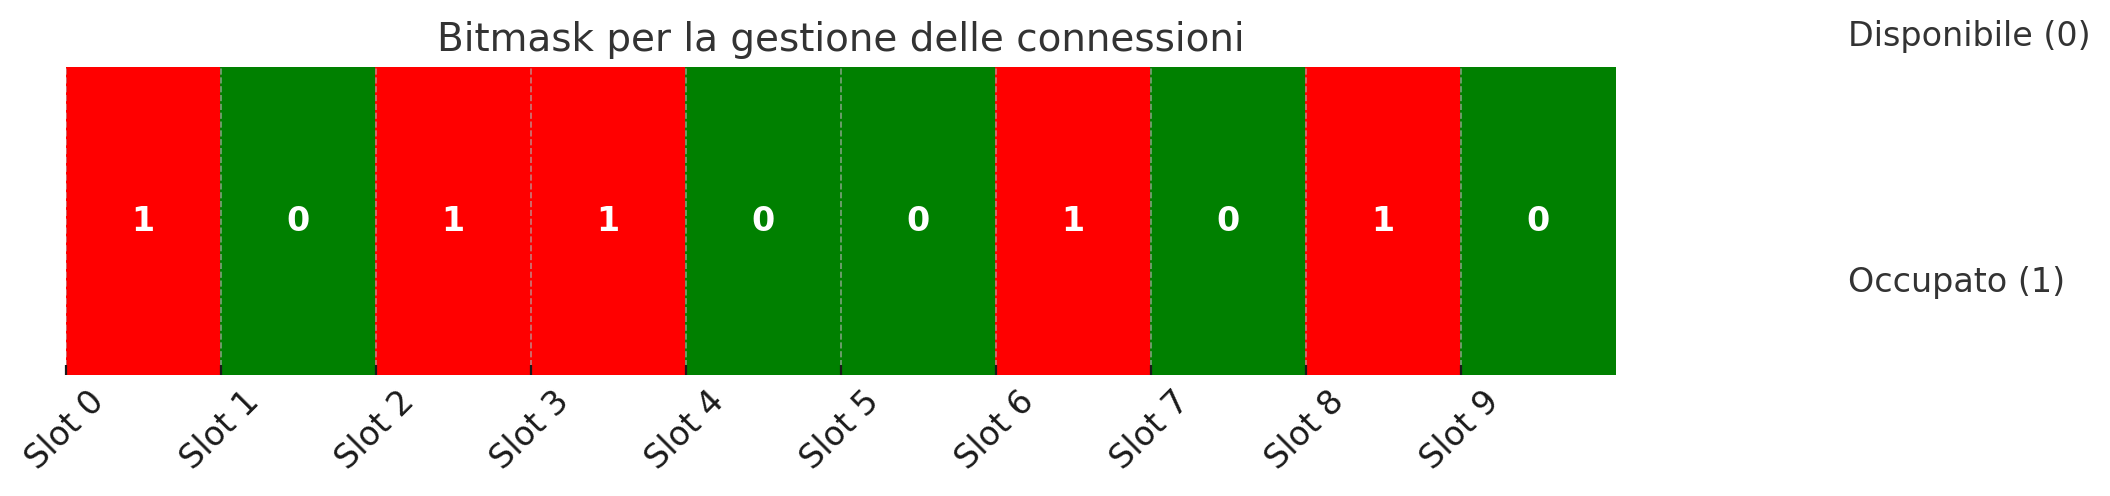
\includegraphics[width=0.75\textwidth]{imgs/01/bitmask.png}
    \caption{Rappresentazione grafica della bitmask.}
    \label{fig:bitmask}
\end{figure}

dove ogni bit della bitmask rappresenta un generico client connesso o meno al server.
Poichè si è scelto di poter accogliere al massimo $2727$ client, la bitmask è stata dimensionata per contenere $2727$ bit.
Questo implica che la dimensione della memoria condivisa, creata con le API di System V IPC, è di $341$ byte, calcolata come segue:

\begin{equation}
    \frac{2727}{8} = 341 \text{ byte} \nonumber
\end{equation}

\subsection{Casi particolari \emoji{police-car-light}}
Sia i client che il server sono dotati di handler per la gestione dei segnali, come \lstinlinebg{SIGINT} e \lstinlinebg{SIGQUIT}, garantendo una terminazione e una pulizia corretta delle risorse, sia nel caso in cui viene terminato prima il client, sia nel caso in cui viene terminato prima il server.
Inoltre è stato gestito il caso in cui il server è down e un generico client tenta di connettersi.
In questo caso il client termina l'esecuzione dopo tre tentativi di connessione falliti.
Per ultimo è stato gestito il caso in cui il server è occupato, ovvero tutti gli slot sono occupati, in questo caso il server notifica il client e quest'ultimo termina l'esecuzione.

\subsection{Timeout di inattività \emoji{three-oclock}}
L'applicazione prevede un meccanismo di timeout per la chiusura automatica delle connessioni inattive.
Si è considerato un tempo di inattività di 3600 secondi (1 ora) come limite massimo di tempo per la connessione.
Se un client non invia alcun messaggio al server per un periodo di tempo superiore a 1 ora, la connessione viene chiusa automaticamente dal server.
Questo meccanismo previene la persistenza di connessioni ``zombie" e garantisce un utilizzo efficiente delle risorse del server.

\subsection{Gestione degli errori e pacchetti persi \emoji{collision}\emoji{package}}
L'applicazione interrompe il trasferimento se si verificano più di $25$ errori consecutivi.
Questo numero è stato scelto per evitare che il protocollo di trasferimento dati entri in uno stato di loop infinito, ad esempio a causa della perdita o corruzione dei pacchetti.
Oltre questo limite, la quantità di dati corrotti renderebbe impossibile la ricostruzione fedele del file, compromettendone l'integrità e l'usabilità.

\subsection{Three-Way Handshake \emoji{handshake}}
Per stabilire una connessione tra client e server, è stato implementato un \textit{Three-Way Handshake} per garantire l'affidabilità e l'integrità della connessione.
Il \textit{Three-Way Handshake} è un protocollo di comunicazione a tre passaggi che consente a due host di stabilire una connessione TCP/IP.
Il protocollo funziona come segue:
\begin{enumerate}
    \item Il client invia un pacchetto di richiesta di connessione al server, contenente il flag \lstinlinebg{SYN} (synchronization request).
    \item Il server risponde con un pacchetto di conferma, contenente il flag \lstinlinebg{SYN} e \lstinlinebg{ACK} (acknowledgment).
    \item Il client invia un pacchetto di conferma al server, contenente il flag \lstinlinebg{ACK}.
    \item La connessione è stabilita e i due host possono iniziare a scambiarsi dati.
\end{enumerate}

\subsubsection{Three-Way Handshake di apertura}
Per la realizzazione del software S.P.Q.R. è stato implementato un \textit{Three-Way Handshake} di apertura per stabilire la connessione tra client e server.
Il client invia un pacchetto di richiesta di connessione al server, contenente il flag \lstinlinebg{SYN}.
Il server risponde con un pacchetto di conferma, contenente il flag \lstinlinebg{SYN-ACK}.
Infine, il client invia un pacchetto di conferma al server, contenente il flag \lstinlinebg{ACK}.
La connessione è stabilita e i due host possono iniziare a scambiarsi dati.

\begin{figure}[h]
    \centering
    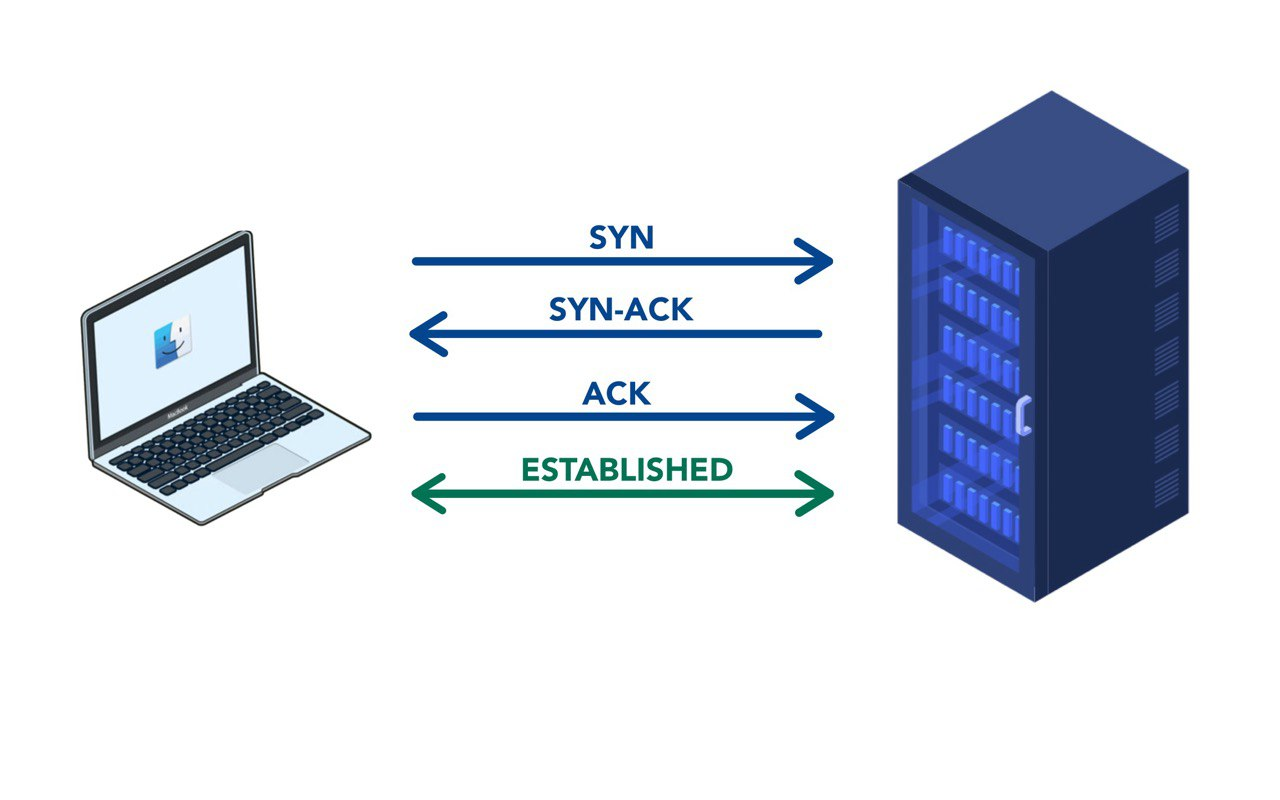
\includegraphics[width=0.65\textwidth]{imgs/02/macbook_server.jpeg}
    \caption{Three-Way Handshake d'apertura.}
\end{figure}

\subsubsection{Three-Way Handshake di chiusura}
Lo stesso vale per il \textit{Three-Way Handshake} di chiusura, che consente a client e server di terminare la connessione in modo sicuro.
Il client invia un pacchetto di richiesta di chiusura al server, contenente il flag \lstinlinebg{FIN}.
Il server risponde con un pacchetto di conferma, contenente il flag \lstinlinebg{FINACK} e invia un pacchetto di conferma al client, contenente il flag \lstinlinebg{FIN}.
Il client risponde con un pacchetto di conferma al server, contenente il flag \lstinlinebg{ACK}.
La connessione è chiusa e i due host possono liberare le risorse allocate.

\begin{figure}[h]
    \centering
    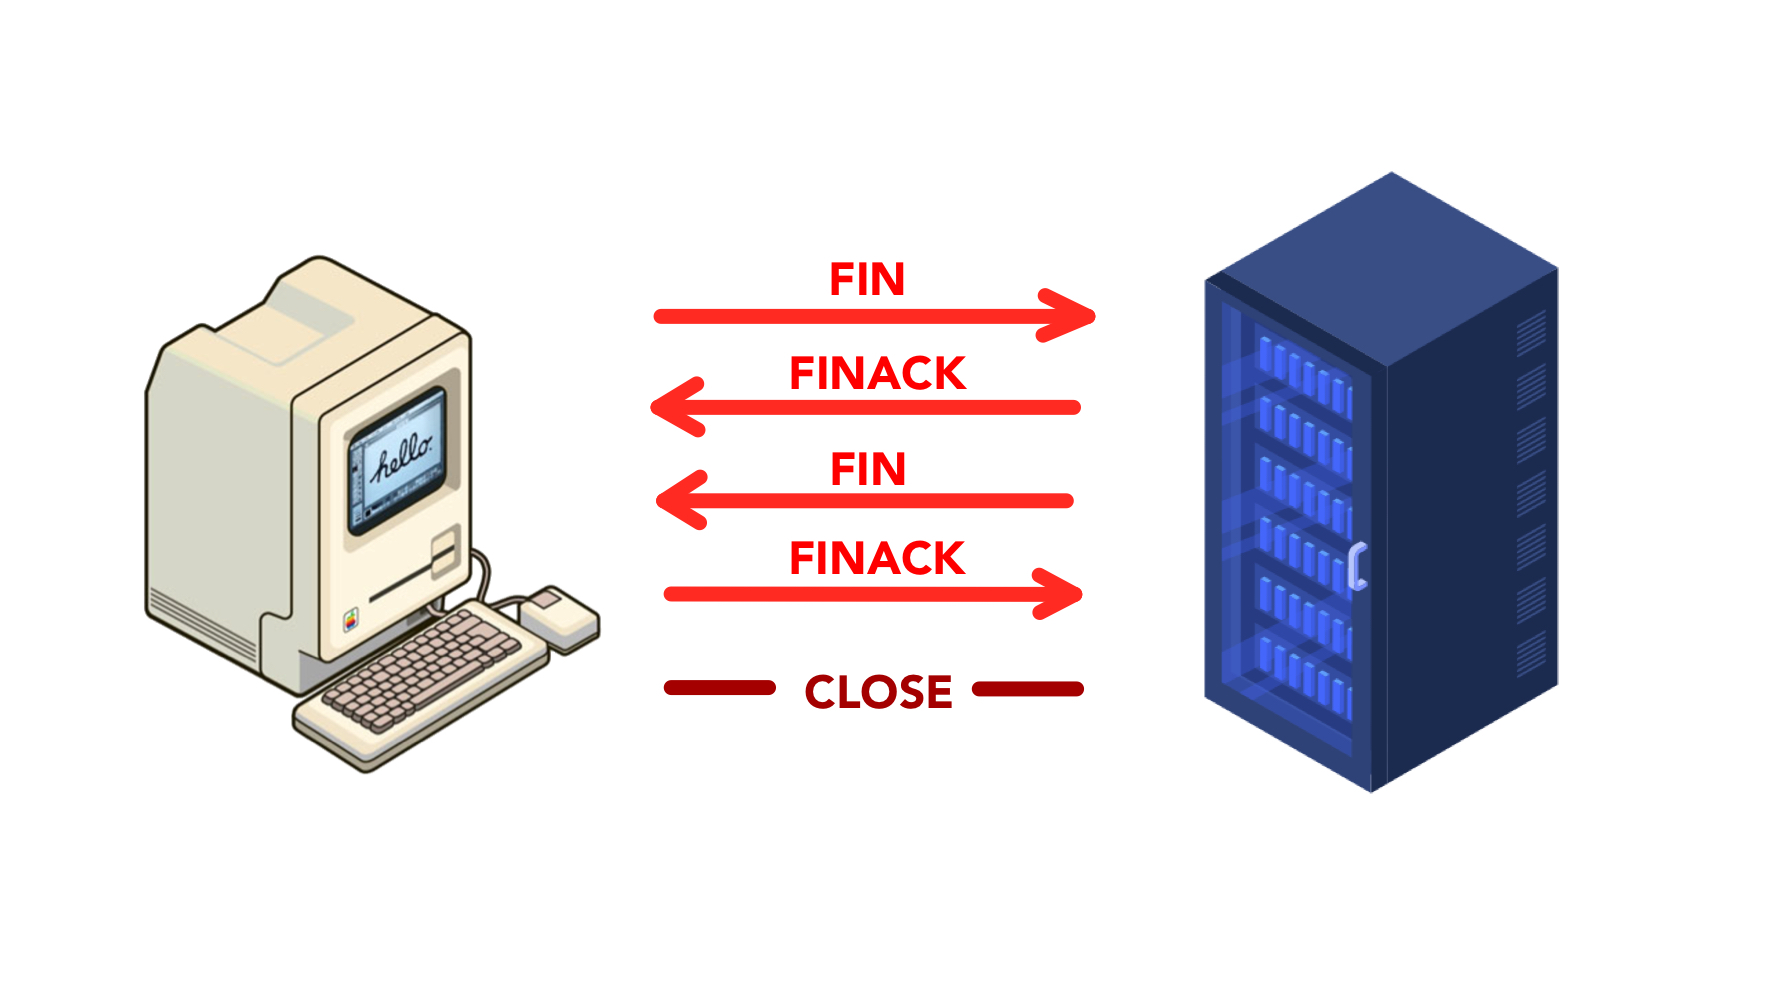
\includegraphics[width=0.65\textwidth]{imgs/02/three-way-handshake-chiusura.jpeg}
    \caption{Three-Way Handshake di chiusura.}
\end{figure}

\subsection{Progressive Bar \emoji{rocket}}
Per rendere il trasferimento dei file più interattivo e coinvolgente, è stata implementata una barra di avanzamento.
La barra di avanzamento mostra la percentuale di completamento del trasferimento, aggiornata in tempo reale.
Questo permette all'utente di monitorare il progresso del trasferimento e di avere un'idea chiara del tempo rimanente.

\begin{figure}[ht]
    \centering
    \animategraphics[autoplay,loop,width=0.95\textwidth]{100}{image/progressive-bar-}{0}{151}
    \caption{Animazione della progressive bar.}
\end{figure}

\chapter{Descrizione dell'implementazione}

In questo capitolo saranno illustrate nel dettaglio le scelte progettuali, con particolare enfasi sull'implementazione, e le soluzioni tecniche adottate nello sviluppo del software S.P.Q.R. (\textit{Selective Protocol for Quality and Reliability}).
Attraverso un'analisi strutturata, verranno presentati i componenti fondamentali del sistema, con particolare attenzione agli aspetti critici che ne garantiscono l'efficienza e l'affidabilità.
Infine saranno analizzate le limitazioni riscontrate durante lo sviluppo.

% Three-Way Handshake:
% - client_open_connection_with_server (Three way handshake apertura)
% - client_close_connection_with_server (Three way handshake chiusura)
% - server_open_connection_with_client (Three way handshake apertura)
% - server_close_connection_with_client (Three way handshake chiusura)
% - send_packet / receive_packet

% SELECTIVE REPEAT:
% - init_packet_loss_simulator
% - can_send_packet
% - receive_data_from_sender
% - main_receiver
% - send_data_to_receiver
% - wait_ack
% - main_sender

\section{Implementazione del server}
Il server è il cuore del sistema, responsabile della gestione delle connessioni con i client, dell'elaborazione dei comandi e del trasferimento dei file.
Di seguito viene riportato il codice sorgente del server attraverso il quale seguirà una spiegazione dettagliata delle funzioni principali.

\begin{lstlisting}[caption={\lstinlinebg{src/server.c}},language=C,escapeinside={(*}{*)},keywords={include, int32_t, void, setup_signal_handling, server_create_socket, load_ascii_art, server_manage_client_connections, PARENT, PORT, puts, return}]
#include "spqr_server.h"

int32_t main(void) {
    setup_signal_handling(PARENT);
    
    int32_t sockfd = server_create_socket(PORT - 1);
    
    load_ascii_art();
    puts("(*\emoji{globe-with-meridians}*) Server is listening for incoming connections.");
    
    return server_manage_client_connections(sockfd);
}
\end{lstlisting}

Analizziamo la prima funzione, \lstinlinebg{setup_signal_handling()}, che si occupa di settare i gestori dei segnali per il processo padre del server.
Si noti che quest'ultima può essere usata anche per il processo figlio, in base al parametro passato.

\begin{lstlisting}[caption={\lstinlinebg{src/spqr_server.c}},language=C,escapeinside={(*}{*)},keywords={sigaction, parent_server_signal_handler, child_server_signal_handler, SIGTERM, sigfillset, sigdelset, sigprocmask, SIG_BLOCK, sizeof, spqr_assert, sigemptyset, if, else, CHILD, NULL, SIGINT, SIGQUIT, struct, sigset_t, memset, signal_handler_t, int32_t, void, server_create_socket, load_ascii_art, server_manage_client_connections, PARENT, PORT, puts, return}]
void setup_signal_handling(signal_handler_t type) {
    struct sigaction sa;
    sigset_t set;

    memset(&sa, 0, sizeof(sa));
    sa.sa_flags = 0;
    spqr_assert(sigemptyset(&sa.sa_mask), "sigemptyset");

    if (type == PARENT) {
        sa.sa_handler = parent_server_signal_handler;
        spqr_assert(sigaction(SIGINT, &sa, NULL), "sigaction");
        spqr_assert(sigaction(SIGQUIT, &sa, NULL), "sigaction");

    } else if (type == CHILD) {
        sa.sa_handler = child_server_signal_handler;
        spqr_assert(sigaction(SIGTERM, &sa, NULL), "sigaction");

        // ? Block all signals except SIGTERM
        spqr_assert(sigfillset(&set), "sigfillset");
        spqr_assert(sigdelset(&set, SIGTERM), "sigdelset");
    }

    spqr_assert(sigprocmask(SIG_BLOCK, &set, NULL), "sigprocmask");
}
\end{lstlisting}

All'interno della funzione \lstinlinebg{setup_signal_handling()} vengono inizializzate le strutture necessarie per la gestione dei segnali, in particolare vengono settati i gestori dei segnali per i segnali \lstinlinebg{SIGINT} e \lstinlinebg{SIGQUIT} nel caso del processo padre, mentre per il processo figlio viene settato il gestore per il segnale \lstinlinebg{SIGTERM}.
Di seguito sono riportate le implementazioni delle funzioni \lstinlinebg{parent_server_signal_handler()} e \lstinlinebg{child_server_signal_handler()}.

\begin{lstlisting}[caption={\lstinlinebg{src/spqr_server.c}},language=C,escapeinside={(*}{*)},keywords={exit, puts, EXIT_SUCCESS, waitpid, shmdt, shmctl, IPC_RMID, SPQR_CLOSE_CONNECTION, const, sigaction, for, uint32_t, MAX_CLIENTS, INVALID_PID, kill, ifdef, DEBUG, endif, SIGTERM, sigfillset, sigdelset, sigprocmask, SIG_BLOCK, sizeof, spqr_assert, sigemptyset, if, char, MAX_READ_LINE, server_receive_packet, server_close_connection_with_client, close, else, CHILD, NULL, SIGINT, SIGQUIT, struct, sigset_t, memset, signal_handler_t, int32_t, void, server_create_socket, load_ascii_art, server_manage_client_connections, PARENT, PORT, printf, return}]
void parent_server_signal_handler(const int32_t signo) {
    if (signo == SIGINT || signo == SIGQUIT) {

    #ifdef DEBUG
        printf("\n[DEBUG (*\emoji{beetle}*)] Server terminated due to %s.\n", signo == SIGINT ? "SIGINT" : "SIGQUIT");
    #endif

        for (uint32_t i = 0; i < MAX_CLIENTS; ++i) {
            if (child_pids[i] != INVALID_PID) {
                kill(child_pids[i], SIGTERM);
            }
        }

        for (uint32_t i = 0; i < MAX_CLIENTS; ++i) {
            if (child_pids[i] != INVALID_PID) {
                waitpid(child_pids[i], NULL, 0);
            #ifdef DEBUG
                printf("[DEBUG (*\emoji{beetle}*)] Child process #%d terminated.\n", i);
            #endif
            }

            if (i == MAX_CLIENTS - 1) {
                spqr_assert(shmdt(shm_bitmask), "shmdt");
                spqr_assert(shmctl(shm_id, IPC_RMID, NULL), "shmctl");
            }
            
            child_pids[i] = INVALID_PID;
        }

        puts(SPQR_CLOSE_CONNECTION);
        exit(EXIT_SUCCESS);
    }
}

void child_server_signal_handler(const int32_t signo) {
    if (signo == SIGTERM) {
        char dummy[MAX_READ_LINE];
        server_receive_packet(dummy, child_sockfd, MAX_READ_LINE);
        memset(dummy, 0, MAX_READ_LINE);
        server_close_connection_with_client(child_sockfd);
        spqr_assert(close(child_sockfd), "close");
        exit(EXIT_SUCCESS);
    }
}
\end{lstlisting}

La seconda funzione di interesse è \lstinlinebg{server_manage_client_connections()}.
I punti salienti riguardanti tale funzione sono la stabilizzazione della connessione e l'assegnazione di una porta dedicata per ogni client, la gestione dei processi figli, la pulizia dei processi zombie, l'utilizzo della funzione \lstinlinebg{select()} per gestire le connessioni in arrivo, la gestione dei segnali e la gestione dei comandi inviati dai client.

\begin{lstlisting}[caption={\lstinlinebg{src/spqr_server.c}},language=C,escapeinside={(*}{*)},keywords={for, get_bit, set_bit, continue, printf, pid_t, setup_signal_handling, init_packet_loss_simulator, EXIT_SUCCESS, exit, WNOHANG, SPQR_SERVER_BUSY, int8_t, const, uint16_t, char, memset, sizeof, key_t, KEY_PATH, ftok, shmget, SHM_SIZE, IPC_CREAT, PERMS, uint8_t, shmat, spqr_assert_shm, FREE, BUSY, fd_set, FD_ZERO, FD_SET, while, true, struct, timeval, select, EINTR, HANDLE_ERROR, break, FD_ISSET, uint32_t, int32_t, void, server_manage_client_commands, server_open_connection_with_client, server_close_connection_with_client, server_receive_packet, server_send_packet, MAX_READ_LINE, MAX_CLIENTS, INVALID_PID, fork, if, else, return, close, waitpid, NULL, spqr_assert, server_create_socket, load_ascii_art, PARENT, PORT, puts}]
int8_t server_manage_client_connections(const int32_t sockfd) {
    uint16_t port;
    char buffer[MAX_READ_LINE];
    memset(buffer, 0, sizeof(buffer));

    // ? Initialize shared memory and bitmask as before
    key_t key = ftok(KEY_PATH, 's');
    spqr_assert(key, "ftok");
    
    shm_id = shmget(key, SHM_SIZE, IPC_CREAT | PERMS);
    spqr_assert(shm_id, "shmget");
    
    shm_bitmask = (uint8_t *)shmat(shm_id, NULL, 0);
    spqr_assert_shm(shm_bitmask, "shmat");
    memset(shm_bitmask, FREE, SHM_SIZE);
    
    memset(child_pids, INVALID_PID, sizeof(child_pids));

    // ? Set up the file descriptor set.
    fd_set read_fds, master_fds;
    int32_t max_fd = sockfd;
    
    FD_ZERO(&master_fds);
    FD_SET(sockfd, &master_fds);

    // ? Main server loop.
    while (true) {
        read_fds = master_fds;
        
        // ? Set timeout for select
        struct timeval timeout;
        timeout.tv_sec = 1;
        timeout.tv_usec = 0;

        int32_t ready = select(max_fd + 1, &read_fds, NULL, NULL, &timeout);
        if (ready < 0) {
            if (errno == EINTR) continue; // ? Handle interruption by signal.
            HANDLE_ERROR("select");
            break;
        }

        // ? Check for new connections on the main socket.
        if (FD_ISSET(sockfd, &read_fds)) {
            if (server_open_connection_with_client(sockfd)) {
                uint32_t no_client = 0;
                for (; no_client < MAX_CLIENTS; ++no_client) {
                    if (!get_bit(no_client)) {
                        set_bit(no_client, BUSY);
                        break;
                    }
                    
                    if (no_client == MAX_CLIENTS - 1) {
                        server_send_packet(SPQR_SERVER_BUSY, sockfd);
                        continue;
                    }
                }

                port = PORT + no_client;
                memset(buffer, 0, sizeof(buffer));
                spqr_assert(snprintf(buffer, sizeof(buffer), "%d", port), "snprintf");
                server_send_packet(buffer, sockfd);
                printf("\nThe client #%d is connected on port %d.\n", no_client, port);

                pid_t pid = fork();
                spqr_assert(pid, "fork");
                
                if (pid == 0) { // ? Child process.
                    spqr_assert(close(sockfd), "close"); // ? Close the parent's socket because it is not needed.
                    setup_signal_handling(CHILD);
                    init_packet_loss_simulator();
                    
                    child_sockfd = server_create_socket(port);
                    int32_t status = server_manage_client_commands(child_sockfd);
                    
                    set_bit(no_client, FREE);
                    printf("Closed connection for client #%d on port %d with exit code %d.\n", no_client, port, status);
                    
                    exit(status); // ? Close the child process.

                } else { // ? Parent process.
                    child_pids[no_client] = pid;
                }
            }
        }

        // ? Check for zombie processes and clean them up.
        int32_t status;
        pid_t wpid;
        while ((wpid = waitpid(INVALID_PID, &status, WNOHANG)) > 0) {
            // ? Handle terminated child process.
            for (uint32_t i = 0; i < MAX_CLIENTS; ++i) {
                if (child_pids[i] == wpid) {
                    child_pids[i] = INVALID_PID;
                    set_bit(i, FREE);
                    break;
                }
            }
        }
    }

    return EXIT_SUCCESS;
}
\end{lstlisting}

Inoltre, come già accennato nel capitolo precedente, si è implementata una bitmask tramite memoria condivisa per tenere traccia delle connessioni attive.
In particolare le funzioni \lstinlinebg{set_bit()} e \lstinlinebg{get_bit()} sono fondamentali per la gestione della bitmask.

\begin{lstlisting}[caption={\lstinlinebg{src/spqr_server.c}},language=C,keywords={const, int8_t, bitmask_t, CHAR_BIT, fopen, exit, printf, if, else, return, stdin, void,  set_seconds_timeout, sockfd, MAX_CLIENTS, SIGQUIT, SIGINT, int32_t, uint32_t, INVALID_PID, SIGTERM, EXIT_SUCCESS, BUSY}]
void set_bit(const uint32_t client_id, const bitmask_t state) {
    int32_t byte_index = client_id / CHAR_BIT;
    int32_t bit_index = client_id % CHAR_BIT;
    if (state == BUSY) {
        shm_bitmask[byte_index] |= (1 << bit_index); // ? Set the bit to 1
    } else {
        shm_bitmask[byte_index] &= ~(1 << bit_index); // ? Set the bit to 0
    }
}

int8_t get_bit(const uint32_t client_id) {
    int32_t byte_index = client_id / CHAR_BIT;
    int32_t bit_index = client_id % CHAR_BIT;
    return (shm_bitmask[byte_index] >> bit_index) & 1;
}
\end{lstlisting}

Infine, una volta che un client si connette al server, viene creato un processo figlio per gestire la connessione tramite la funzione \lstinlinebg{server_manage_client_commands()}.
Quest'ultima ha il compito di gestire i comandi inviati dal client, in particolare i comandi \lstinlinebg{GET} e \lstinlinebg{PUT} per il trasferimento dei file e i comandi \lstinlinebg{LIST} e \lstinlinebg{CLOSE} per la visualizzazione dei file e la chiusura della connessione.

\section{Implementazione del client}
Il client è il componente che si occupa di stabilire la connessione con il server, inviare i comandi e ricevere/inviare i file richiesti.
Di seguito viene riportato il codice sorgente del client attraverso il quale seguirà una spiegazione dettagliata delle funzioni principali.

\begin{lstlisting}[caption={\lstinlinebg{src/client.c}},language=C,escapeinside={(*}{*)},keywords={if, client_manage_server_commands, WINDOW_SIZE, LOSS_PROBABILITY, TIMEOUT, ADAPTIVE, close, load_ascii_art, printf, INFO, spqr_free, spqr_assert, MAX_READ_LINE, spqr_assert_ptr, memset, init_packet_loss_simulator, malloc, fprintf, stderr, EXIT_FAILURE, const, char, int32_t, void, setup_signal_handling, client_create_socket, client_establish_connection_with_server, client_manage_server_commands, PARENT, PORT, puts, return, include}]
#include "spqr_client.h"

int32_t main(int32_t argc, const char **argv) {
    if (argc != 2) {
        fprintf(stderr, "Usage: %s <IPv4>\n", *argv);
        return EXIT_FAILURE;
    }

    setup_signal_handling();

    init_packet_loss_simulator();

    server_response = malloc(MAX_READ_LINE);
    spqr_assert_ptr(server_response, "malloc");
    memset(server_response, 0, MAX_READ_LINE);

    if (!client_establish_connection_with_server(argv[1])) {
        spqr_free(&server_response);
        spqr_assert(close(sockfd), "close");
        return EXIT_FAILURE;
    }

    load_ascii_art();
    printf("(*\emoji{globe-with-meridians}*) Connection established with the server.\n");
    printf(INFO, WINDOW_SIZE, LOSS_PROBABILITY, TIMEOUT, ADAPTIVE ? "true" : "false");

    return client_manage_server_commands();
}
\end{lstlisting}

Di particolare interesse è la funzione \lstinlinebg{setup_signal_handling()} che si occupa di settare i gestori dei segnali per il client.

\begin{lstlisting}[caption={\lstinlinebg{src/spqr_client.c}},language=C,escapeinside={(*}{*)},keywords={SIGALRM, sigaction, client_signal_handler, SIGTERM, sigfillset, sigdelset, sigprocmask, SIG_BLOCK, sizeof, spqr_assert, sigemptyset, if, else, NULL, SIGINT, SIGQUIT, struct, sigset_t, memset, signal_handler_t, int32_t, void, client_create_socket, client_establish_connection_with_server, client_manage_server_commands, PARENT, PORT, puts, return}]
void setup_signal_handling(void) {
    struct sigaction sa;
    sigset_t set;

    memset(&sa, 0, sizeof(sa));
    sa.sa_handler = client_signal_handler;
    sa.sa_flags = 0;
    spqr_assert(sigemptyset(&sa.sa_mask), "sigemptyset");
    spqr_assert(sigaction(SIGINT, &sa, NULL), "sigaction");
    spqr_assert(sigaction(SIGQUIT, &sa, NULL), "sigaction");
    spqr_assert(sigaction(SIGALRM, &sa, NULL), "sigaction");
    
    // ? Block all signals except SIGINT, SIGQUIT, SIGALRM.
    spqr_assert(sigfillset(&set), "sigfillset");
    spqr_assert(sigdelset(&set, SIGINT), "sigdelset");
    spqr_assert(sigdelset(&set, SIGQUIT), "sigdelset");
    spqr_assert(sigdelset(&set, SIGALRM), "sigdelset");
    spqr_assert(sigprocmask(SIG_BLOCK, &set, NULL), "sigprocmask");
}
\end{lstlisting}

dove \lstinlinebg{client_signal_handler()} è la funzione che si occupa di gestire i segnali inviati al client.

\begin{lstlisting}[caption={\lstinlinebg{src/spqr_client.c}},language=C,escapeinside={(*}{*)},keywords={if, else, spqr_assert, client_send_packet, client_close_connection_with_server, const, SPQR_SESSION_STOPPED, ifdef, endif, DEBUG, exit, puts, EXIT_SUCCESS, spqr_free, close, sockfd, SIGINT, SIGQUIT, SIGALRM, signal_handler_t, int32_t, void, client_create_socket, client_establish_connection_with_server, client_manage_server_commands, PARENT, PORT, return}]
void client_signal_handler(const int32_t sig) {
    if (sig == SIGINT) {
    #ifdef DEBUG
        puts("\n" SPQR_SESSION_STOPPED);
    #endif
        client_send_packet(feedback.EXIT, sockfd);
        client_close_connection_with_server(sockfd);

    } else if (sig == SIGQUIT) {
    #ifdef DEBUG
        puts("\n" SPQR_SESSION_STOPPED);
    #endif
        client_send_packet(feedback.EXIT, sockfd);

    } else if (sig == SIGALRM) {
        puts("\n" SPQR_TIMEOUT_SESSION);

        client_send_packet(feedback.EXIT, sockfd);
        client_close_connection_with_server(sockfd);
    }

    spqr_free(&server_response);
    spqr_free(&client_pathname);
    spqr_assert(close(sockfd), "close");

    exit(EXIT_SUCCESS);
}
\end{lstlisting}

Un altra funzione di interesse è \lstinlinebg{client_establish_connection_with_server()}, la quale si occupa di stabilire la connessione con il server.

\begin{lstlisting}[caption={\lstinlinebg{src/spqr_client.c}},language=C,escapeinside={(*}{*)},keywords={continue, break, CONNECTION_ATTEMPTS, HANDLE_ERROR, if, int8_t, char, true, false, COLOR_RESET,  else, spqr_assert, client_send_packet, client_close_connection_with_server, const, client_open_connection_with_server, MAX_READ_LINE, uint16_t, to_uint16, SPQR_CONNECTION_REFUSED, SPQR_SESSION_STOPPED, ifdef, endif, DEBUG, exit, puts, strcmp, SPQR_SERVER_BUSY, EXIT_SUCCESS, spqr_free, close, while, printf, COLOR_RED, client_receive_packet, set_seconds_timeout, SIGINT, SIGQUIT, SIGALRM, signal_handler_t, int32_t, void, client_create_socket, bool, client_manage_server_commands, PARENT, PORT, return}]
bool client_establish_connection_with_server(const char *ip) {
    int8_t connection_attempts = CONNECTION_ATTEMPTS;

    sockfd = client_create_socket(ip, PORT - 1);
    spqr_assert(sockfd, "client_create_socket");

    set_seconds_timeout(sockfd, CONNECTION_ATTEMPTS);
    while (connection_attempts > 0) {
        if (!client_open_connection_with_server(sockfd)) {
            printf(COLOR_RED "(*\emoji{warning}*) Connection refused (remaining attempts: %d)\n", --connection_attempts);
            continue;
        }
        set_seconds_timeout(sockfd, 0);
        
        client_receive_packet(server_response, sockfd, MAX_READ_LINE);
        if (strcmp(server_response, SPQR_SERVER_BUSY) == 0) {
            puts(SPQR_SERVER_BUSY);
            return false;
        }

        uint16_t port;
        if (!to_uint16(server_response, &port)) {
        #ifdef DEBUG
            HANDLE_ERROR("to_uint16");
        #endif
            return false;
        }
        
        spqr_assert(close(sockfd), "close");
        sockfd = client_create_socket(ip, port);
        break;
    }
    set_seconds_timeout(sockfd, 0);

    if (connection_attempts == 0) {
        puts(COLOR_RESET SPQR_CONNECTION_REFUSED);
        return false;
    }

    puts(COLOR_RESET);
    return true;
}
\end{lstlisting}

In particolare essa gestisce i tentativi di connessione e il caso in cui il server è down.
Infatti, in quest'ultimo caso il client tenterà di connettersi nuovamente per un numero di volte definito dalla costante \lstinlinebg{CONNECTION_ATTEMPTS} che per default è settata a $3$.
Per fare ciò è usato un timeout, tramite la funzione \lstinlinebg{set_seconds_timeout()}, per evitare che il client rimanga bloccato in attesa di una risposta dal server.
Quindi, se il server è down, il client stamperà un messaggio di errore e terminerà la connessione.
Infine, la funzione \lstinlinebg{client_manage_server_commands()} è responsabile della gestione dei comandi (\lstinlinebg{GET}, \lstinlinebg{PUT}, \lstinlinebg{LIST} e \lstinlinebg{CLOSE}) inviati dal server al client.

\section{Implementazione del Three-Way Handshake}
Il \textit{Three-Way Handshake} di apertura, il cui funzionamento è stato descritto nel capitolo precedente, è stato implementato tramite le funzioni \lstinlinebg{server_open_connection_with_client()} e \lstinlinebg{client_open_connection_with_server()} per il server e il client rispettivamente.

\begin{lstlisting}[caption={\lstinlinebg{src/spqr_server.c}},language=C,escapeinside={(*}{*)},keywords={bool, memset, ifdef, endif, HANDLE_ERROR, DEBUG, return, strcmp, true, false, if, else, spqr_assert, client_send_packet, client_receive_packet, const, char, int32_t, void, server_send_packet, server_receive_packet, MAX_READ_LINE, SPQR_SYN, SPQR_ACK, SPQR_SYN_ACK, SPQR_ACK_ACK}]
bool server_open_connection_with_client(const int32_t sockfd) {
    char buffer[MAX_READ_LINE];
    memset(buffer, 0, MAX_READ_LINE);

    server_receive_packet(buffer, sockfd, MAX_READ_LINE);
    if (strcmp(buffer, udp.SYN)) {
    #ifdef DEBUG
        HANDLE_ERROR(udp.SYN);
    #endif
        return false;
    }

    server_send_packet(udp.SYNACK, sockfd);

    server_receive_packet(buffer, sockfd, MAX_READ_LINE);
    if (strcmp(buffer, udp.ACK)) {
    #ifdef DEBUG
        HANDLE_ERROR(udp.ACK);
    #endif
        return false;
    }

    return true;
}
\end{lstlisting}

\begin{lstlisting}[caption={\lstinlinebg{src/spqr_client.c}},language=C,escapeinside={(*}{*)},keywords={if, else, ifdef, endif, DEBUG, memset, strcmp, bool, HANDLE_ERROR, return, false, true, spqr_assert, client_send_packet, client_receive_packet, const, char, int32_t, void, server_send_packet, server_receive_packet, MAX_READ_LINE, SPQR_SYN, SPQR_ACK, SPQR_SYN_ACK, SPQR_ACK_ACK}]
bool client_open_connection_with_server(const int32_t sockfd) {
    char buffer[MAX_READ_LINE];
    memset(buffer, 0, MAX_READ_LINE);

    client_send_packet(udp.SYN, sockfd);

    client_receive_packet(buffer, sockfd, MAX_READ_LINE);
    if (strcmp(buffer, udp.SYNACK)) {
    #ifdef DEBUG
        HANDLE_ERROR(udp.SYNACK);
    #endif
        return false;
    }

    client_send_packet(udp.ACK, sockfd);
    
    return true;
}
\end{lstlisting}


Mentre il \textit{Three-Way Handshake} di chiusura è stato implementato tramite le funzioni \lstinlinebg{server_close_connection_with_client()} e \lstinlinebg{client_close_connection_with_server()} per il server e il client rispettivamente.

\begin{lstlisting}[caption={\lstinlinebg{src/spqr_server.c}},language=C,escapeinside={(*}{*)},keywords={int8_t, memset, strcmp, return, EXIT_SUCCESS, TRANSFER_ERROR, HANDLE_ERROR, ifdef, endif, DEBUG, if, else, spqr_assert, client_send_packet, client_receive_packet, const, char, int32_t, void, server_send_packet, server_receive_packet, MAX_READ_LINE, SPQR_SYN, SPQR_ACK, SPQR_SYN_ACK, SPQR_ACK_ACK}]
int8_t server_close_connection_with_client(const int32_t sockfd) {
    char buffer[MAX_READ_LINE];
    memset(buffer, 0, MAX_READ_LINE);

    server_receive_packet(buffer, sockfd, MAX_READ_LINE);
    if (strcmp(buffer, udp.FIN)) {
    #ifdef DEBUG
        HANDLE_ERROR(udp.FIN);
    #endif
        return TRANSFER_ERROR;
    }
    
    server_send_packet(udp.FINACK, sockfd);
    server_send_packet(udp.FIN, sockfd);
    
    server_receive_packet(buffer, sockfd, MAX_READ_LINE);
    if (strcmp(buffer, udp.FINACK)) {
    #ifdef DEBUG
        HANDLE_ERROR("FINACK");
    #endif
        return TRANSFER_ERROR;
    }

    return EXIT_SUCCESS;
}
\end{lstlisting}

\begin{lstlisting}[caption={\lstinlinebg{src/spqr_client.c}},language=C,escapeinside={(*}{*)},keywords={SPQR_CLOSE_CONNECTION, int8_t, memset, strcmp, ifdef, endif, DEBUG, return, HANDLE_ERROR, TRANSFER_ERROR, puts, EXIT_SUCCESS, if, else, spqr_assert, client_send_packet, client_receive_packet, const, char, int32_t, void, server_send_packet, server_receive_packet, MAX_READ_LINE, SPQR_SYN, SPQR_ACK, SPQR_SYN_ACK, SPQR_ACK_ACK}]
int8_t client_close_connection_with_server(const int32_t sockfd) {
    char buffer[MAX_READ_LINE];
    memset(buffer, 0, MAX_READ_LINE);

    client_send_packet(udp.FIN, sockfd);

    client_receive_packet(buffer, sockfd, MAX_READ_LINE);
    if (strcmp(buffer, udp.FINACK)) {
    #ifdef DEBUG
        HANDLE_ERROR(udp.FINACK);
    #endif
        return TRANSFER_ERROR;
    }

    client_receive_packet(buffer, sockfd, MAX_READ_LINE);
    if (strcmp(buffer, udp.FIN)) {
    #ifdef DEBUG
        HANDLE_ERROR(udp.FIN);
    #endif
        return TRANSFER_ERROR;
    }
    
    client_send_packet(udp.FINACK, sockfd);
    puts(SPQR_CLOSE_CONNECTION);
    return EXIT_SUCCESS;
}
\end{lstlisting}

Infine si riportano le implementazioni dettagliate delle funzioni \lstinlinebg{server_receive_packet()}, \lstinlinebg{server_send_packet()}, \lstinlinebg{client_send_packet()} e \lstinlinebg{client_receive_packet()}.

\begin{lstlisting}[caption={\lstinlinebg{src/spqr_server.c}},language=C,escapeinside={(*}{*)},keywords={strlen, uint64_t, MSG_WAITALL, struct, sockaddr, recvfrom, if, else, spqr_assert, sendto, const, char, int32_t, void, MAX_READ_LINE, udp, sockaddr_in, memset, sizeof, inet_pton, htons, perror, return}]
char *server_receive_packet(char *msg, const int32_t sockfd, const uint64_t size) {
    memset(msg, 0, size);
    spqr_assert(recvfrom(sockfd, msg, size, MSG_WAITALL, (struct sockaddr *) &client_addr, &client_len), "recvfrom");
    return msg;
}

void server_send_packet(const char *msg, const int32_t sockfd) {
    spqr_assert(sendto(sockfd, msg, strlen(msg), 0, (struct sockaddr *) &client_addr, client_len), "sendto");
}
\end{lstlisting}

\begin{lstlisting}[caption={\lstinlinebg{src/spqr_client.c}},language=C,escapeinside={(*}{*)},keywords={strlen, uint64_t, int64_t, recvfrom, struct, sockaddr, HANDLE_ERROR, EWOULDBLOCK, EAGAIN, ifdef, endif, DEBUG, MSG_WAITALL, if, else, spqr_assert, sendto, const, char, int32_t, void, client_send_packet, MAX_READ_LINE, udp, sockaddr_in, memset, sizeof, inet_pton, htons, perror, return}]
void client_send_packet(const char *msg, const int32_t sockfd) {
    spqr_assert(sendto(sockfd, msg, strlen(msg), 0, (struct sockaddr *) &server_addr, server_len), "sendto");
}

char *client_receive_packet(char *msg, const int32_t sockfd, const uint64_t size) {
    memset(msg, 0, size);
    int64_t n = recvfrom(sockfd, msg, size, MSG_WAITALL, (struct sockaddr *) &server_addr, &server_len);
    if (n < 0) {
        if (errno == EWOULDBLOCK || errno == EAGAIN) {
            return NULL;

        } else {
        #ifdef DEBUG
            HANDLE_ERROR("recvfrom");
        #endif
        }
    }
    return msg;
}
\end{lstlisting}

\section{Implementazione del protocollo Selective Repeat}
Per l'implementazione del protocollo \textit{Selective Repeat} sono state implementate due strutture dati, \lstinlinebg{packet_t} e \lstinlinebg{ack_packet_t}, per rappresentare i pacchetti e i pacchetti di ack rispettivamente.

\begin{lstlisting}[caption={\lstinlinebg{src/protocol.h}},language=C,escapeinside={(*}{*)},keywords={ack_packet_t, packet_t, bool, int8_t, int32_t, int64_t, define, PACKET_SIZE, MAX_RETRIES, typedef, struct, uint32_t, uint16_t, uint8_t, char, spqr_packet_t, spqr_ack_t}]
#define PACKET_SIZE 1500 // ? bytes

typedef struct {
    int8_t payload[PACKET_SIZE]; // ? Data payload
    int32_t seq_num;             // ? Sequence number
    int32_t no_packets_to_send;  // ? Total number of packets to send
    int64_t no_bytes_to_send;    // ? Total number of bytes to send
    int64_t size;                // ? Size of the packet
    bool sent;                   // ? Sent flag
    bool received;               // ? Received flag
    bool ack;                    // ? Acknowledged flag
} packet_t;

typedef struct {
    int32_t seq_num;    // ? Sequence number
    int64_t size;       // ? Size of the packet
    int64_t write_byte; // ? Number of bytes written
} ack_packet_t;
\end{lstlisting}

\subsection{Implementazione del sender}
Il sender è responsabile dell'invio dei pacchetti e della gestione degli ack ricevuti.
In questo caso particolare sono state implementate tre funzioni principali: \lstinlinebg{main_sender()}, \lstinlinebg{send_data_to_receiver()} e \lstinlinebg{wait_ack()}.
La funzione \lstinlinebg{main_sender()} si occupa di configurare il timeout del socket, di aprire e leggere il file da inviare, di calcolare la dimensione del file e il numero di pacchetti da inviare, di inizializzare la finestra di invio, di coordinare l'invio dei pacchetti e la gestione degli ACK.
Inoltre si occupa di calcolare le statistiche di throughput e di stamparle a fine trasmissione.
Infine gestisce gli errori e il fallimento del trasferimento.

\begin{lstlisting}[caption={\lstinlinebg{src/protocol.c}},language=C,keywords={TIMEOUT, fopen, for, fread, PACKET_SIZE, break, ifdef, endif, IS_CLIENT, timeval, gettimeofday, send_data_to_receiver, wait_ack, while, true, ack_packet_t, recvfrom, WRITE_BYTE_ERROR, MAX_ERRORS, double, SPQR_KB, FILE_TRANSFER_FAILED, EXIT_SUCCESS, FILE_TRANSFER_COMPLETED, printf, sendto, SEQ_NUM_ERROR, sizeof, int8_t, int32_t, uint16_t, int64_t, struct, sockaddr, sockaddr_in, char, socklen_t, uint32_t, uint64_t, WINDOW_SIZE, stat, fstat, fileno, set_timeout, FILE, NULL, HANDLE_ERROR, return, TRANSFER_ERROR, if, else, perror, exit, fprintf, stderr, MAX_RETRIES, spqr_assert, spqr_free, fclose, free, spqr_assert_ptr, fseek, SEEK_END, ftell, rewind, malloc, memset, sizeof, packet_t, MAX_READ_LINE, MAX_WINDOW_SIZE, MAX_PACKETS, MAX_ACKS}]
int8_t main_sender(int32_t sockfd, struct sockaddr_in *sender_addr, char *pathname) {
    socklen_t len = sizeof(*sender_addr);
    int32_t seq_num = 0;
    int64_t n;
    uint16_t max_errors = 0;
    uint64_t counter = 0;
    int32_t no_packets_to_send = 0;

    // ? Set the timeout of the socket.
    set_timeout(sockfd, TIMEOUT);

    // ? Open the file in read-binary mode.
    FILE *file = fopen(pathname, "rb");
    if (file == NULL) {
        HANDLE_ERROR("fopen");
        return TRANSFER_ERROR;
    }

    // ? Calculate the size of the file.
    struct stat st;
    if (fstat(fileno(file), &st) != 0) {
        HANDLE_ERROR("fstat");
        fclose(file);
        return TRANSFER_ERROR;
    }
    int64_t size_file = st.st_size;

    // ? Calculate the number of packets to send.
    no_packets_to_send = (size_file % PACKET_SIZE) ? (size_file / PACKET_SIZE) + 1 : size_file / PACKET_SIZE;

    // ? Create the initial window.
    uint32_t window_size = (no_packets_to_send < WINDOW_SIZE) ? no_packets_to_send : WINDOW_SIZE;
    packet_t window[WINDOW_SIZE] = { 0 };

    // ? Fill the window with the packets.
    for (uint32_t i = 0; i < window_size; ++i) {
        packet_t packet = { 0 };
        
        uint64_t num_read = fread(packet.payload, 1, PACKET_SIZE, file);
        if (num_read == 0) { break; }

        counter += num_read;
        packet.seq_num = seq_num;
        packet.no_packets_to_send = no_packets_to_send;
        packet.no_bytes_to_send = counter;
        packet.size = num_read;
        packet.sent = false;
        packet.ack = false;
        packet.received = false;
        window[i] = packet;

        seq_num = (seq_num + 1) % window_size;
    }

#ifdef IS_CLIENT
    struct timeval end, start;
    spqr_assert(gettimeofday(&start, NULL), "gettimeofday");
#endif

    // ? Start sending the packets.
    send_data_to_receiver(sockfd, sender_addr, window, window_size);
    wait_ack(sockfd, sender_addr, len, window, window_size, file, size_file, &max_errors, &counter, &no_packets_to_send);
    
#ifdef IS_CLIENT
    spqr_assert(gettimeofday(&end, NULL), "gettimeofday");
#endif

    int64_t ret = 0;
    while (true) {
        ack_packet_t new_ack = { 0 };
        n = recvfrom(sockfd, &new_ack, sizeof(new_ack), 0, (struct sockaddr *) sender_addr, &len);
        if (n < 0) { break; }
        ret = new_ack.write_byte;
    }

    spqr_assert(fclose(file), "fclose");
    set_timeout(sockfd, 0);

    if (ret == WRITE_BYTE_ERROR) { return TRANSFER_ERROR; }

#ifdef IS_CLIENT
    double time = end.tv_sec - start.tv_sec + (double)(end.tv_usec - start.tv_usec) / 1e6;
    double throughput = (time != 0.0) ? (size_file / time) / SPQR_KB : 0.0; // [kB/s]
#endif

    if (max_errors >= MAX_ERRORS) {
    
    #ifdef IS_CLIENT
        printf("\n\n" FILE_TRANSFER_FAILED, time, throughput);
    #endif
    
        packet_t packet = { 0 };
        packet.seq_num = SEQ_NUM_ERROR;

        n = sendto(sockfd, &packet, sizeof(packet), 0, (struct sockaddr *) sender_addr, len);
        if (n < 0) { HANDLE_ERROR("sendto"); }
    
        return TRANSFER_ERROR;
    }

#ifdef IS_CLIENT
    printf("\n\n" FILE_TRANSFER_COMPLETED, time, throughput);
#endif

    return EXIT_SUCCESS;
}
\end{lstlisting}

La funzione \lstinlinebg{send_data_to_receiver()} si occupa dell'invio effettivo dei pacchetti al receiver, verificando quali pacchetti nella finestra devono essere inviati.
Inoltre simula l'eventuale perdita di pacchetti tramite l'ausilio della funzione \lstinlinebg{can_send_packet()}.

\begin{lstlisting}[caption={\lstinlinebg{src/common.c}},language=C,keywords={void, LOSS_PROBABILITY, rand, bool, for, fread, PACKET_SIZE, break, ifdef, endif, IS_CLIENT, timeval, gettimeofday, send_data_to_receiver, wait_ack, while, true, ack_packet_t, recvfrom, WRITE_BYTE_ERROR, MAX_ERRORS, double, SPQR_KB, FILE_TRANSFER_FAILED, EXIT_SUCCESS, FILE_TRANSFER_COMPLETED, printf, sendto, SEQ_NUM_ERROR, sizeof, int8_t, int32_t, uint16_t, int64_t, struct, sockaddr, sockaddr_in, char, socklen_t, uint32_t, uint64_t, WINDOW_SIZE, stat, fstat, fileno, set_timeout, FILE, NULL, HANDLE_ERROR, return, TRANSFER_ERROR, if, else, perror, exit, fprintf, stderr, MAX_RETRIES, spqr_assert, spqr_free, fclose, free, spqr_assert_ptr, fseek, SEEK_END, ftell, rewind, malloc, memset, sizeof, packet_t, MAX_READ_LINE, MAX_WINDOW_SIZE, MAX_PACKETS, MAX_ACKS}]
// ? This function is used to simulate the loss of a packet.
// ? The function returns true if the packet can be sent, false otherwise.
bool can_send_packet(void) {
    return (rand() % 100 + 1) > LOSS_PROBABILITY;
}
\end{lstlisting}

Infine marca i pacchetti come inviati e verifica il completamento del trasferimento.

\begin{lstlisting}[caption={\lstinlinebg{src/protocol.c}},language=C,keywords={void, continue, can_send_packet, for, fread, PACKET_SIZE, break, ifdef, endif, IS_CLIENT, false, timeval, gettimeofday, wait_ack, while, true, ack_packet_t, recvfrom, WRITE_BYTE_ERROR, MAX_ERRORS, double, SPQR_KB, FILE_TRANSFER_FAILED, EXIT_SUCCESS, FILE_TRANSFER_COMPLETED, printf, sendto, SEQ_NUM_ERROR, sizeof, int8_t, int32_t, uint16_t, int64_t, struct, sockaddr, sockaddr_in, char, socklen_t, uint32_t, uint64_t, WINDOW_SIZE, stat, fstat, fileno, set_timeout, FILE, NULL, HANDLE_ERROR, return, TRANSFER_ERROR, if, else, perror, exit, fprintf, stderr, MAX_RETRIES, spqr_assert, spqr_free, fclose, free, spqr_assert_ptr, fseek, SEEK_END, ftell, rewind, malloc, memset, sizeof, packet_t, MAX_READ_LINE, MAX_WINDOW_SIZE, MAX_PACKETS, MAX_ACKS}]
void send_data_to_receiver(int32_t sockfd, struct sockaddr_in *sender_addr, packet_t *window, uint32_t window_size) {
    int64_t n;
    for (uint32_t i = 0; i < window_size; ++i) {
        if (window[i].ack == false) { // ? Check if the packet has been acknowledged.
            if (can_send_packet()) { // ? Check if the packet is lost.
                n = sendto(sockfd, &window[i], sizeof(window[i]), 0, (struct sockaddr *) sender_addr, sizeof(*sender_addr));
                if (n < 0) {
                    HANDLE_ERROR("sendto");
                    continue;
                }
                window[i].sent = true;
                if (window[i].size == 0 || n == 0) { break; } // ? Check if the file has been completely sent.
            }
        }
    }
}
\end{lstlisting}

Infine la funzione \lstinlinebg{wait_ack()} attende e gestice gli ACK dal receiver, implementa il meccaniscmo di timeout e ritrasmissione, gestisce il conteggio degli errori, aggiorna la finestra scorrevole, carica nuovi pacchetti quando necessario, implementa il controllo di flusso e gestisce il timeout adattivo se abilitato.

\begin{lstlisting}[caption={\lstinlinebg{src/protocol.c}},language=C,keywords={print_progress, ADAPTIVE, decrease_timeout, increase_timeout, goto, can_send_packet, false, MSG_CONFIRM, for, fread, PACKET_SIZE, break, ifdef, endif, IS_CLIENT, timeval, gettimeofday, send_data_to_receiver, void, while, true, ack_packet_t, recvfrom, WRITE_BYTE_ERROR, MAX_ERRORS, double, SPQR_KB, FILE_TRANSFER_FAILED, EXIT_SUCCESS, FILE_TRANSFER_COMPLETED, printf, sendto, SEQ_NUM_ERROR, sizeof, int8_t, int32_t, uint16_t, int64_t, struct, sockaddr, sockaddr_in, char, socklen_t, uint32_t, uint64_t, WINDOW_SIZE, stat, fstat, fileno, set_timeout, FILE, NULL, HANDLE_ERROR, return, TRANSFER_ERROR, if, else, perror, exit, fprintf, stderr, MAX_RETRIES, spqr_assert, spqr_free, fclose, free, spqr_assert_ptr, fseek, SEEK_END, ftell, rewind, malloc, memset, sizeof, packet_t, MAX_READ_LINE, MAX_WINDOW_SIZE, MAX_PACKETS, MAX_ACKS}]
void wait_ack(int32_t sockfd, struct sockaddr_in *sender_addr, socklen_t len, packet_t *window, uint32_t window_size, FILE *file, int64_t size_file, uint16_t *max_errors, uint64_t *counter, int32_t *no_packets_to_send) {
    int64_t n;
    int32_t ack_num;
    int64_t last_ack_confirmed_bytes = 0;
    uint64_t num_read;
    uint32_t i = 0;
    ack_packet_t new_ack = { 0 };

#ifdef IS_CLIENT
    printf("\n");
#endif

    while (true) {
    wait_for_ack:
        n = recvfrom(sockfd, &new_ack, sizeof(new_ack), 0, (struct sockaddr *) sender_addr, &len); // ? Wait for the acknowledgment from the receiver.
        if (n < 0) { // ? If the acknowledgment is not received.
            (*max_errors)++;
            if (*max_errors >= MAX_ERRORS) { return; }
            if (ADAPTIVE) { increase_timeout(sockfd); }

            // ? Resend the packets that have not been acknowledged.
            for (uint32_t j = 0; j < window_size; ++j) {
                if (window[j].ack == false || window[j].no_bytes_to_send > last_ack_confirmed_bytes) {
                    if (can_send_packet()) { // ? Check if the packet is lost.
                        n = sendto(sockfd, &window[j], sizeof(window[j]), MSG_CONFIRM, (struct sockaddr *) sender_addr, sizeof(*sender_addr));
                        if (n < 0) {
                            HANDLE_ERROR("sendto");
                        } else {
                            window[j].sent = true;
                        }
                    }
                }
            }
            goto wait_for_ack;
        }

        *max_errors = 0;

        // ? Check if the acknowledgment is received.
        if (new_ack.seq_num == SEQ_NUM_ERROR || new_ack.write_byte > size_file || new_ack.write_byte == WRITE_BYTE_ERROR) { return; }
        if (ADAPTIVE) { decrease_timeout(sockfd); }

        ack_num = new_ack.seq_num;
        if (new_ack.size > last_ack_confirmed_bytes) { last_ack_confirmed_bytes = new_ack.size; }

        // ? If the acknowledgment is received, I skip to the next packet.
        if (window[ack_num].ack == true) {
            continue;

        } else {
            window[ack_num].ack = true;
        
        #ifdef IS_CLIENT
            print_progress(size_file, new_ack.write_byte);
        #endif

            while (window[i].ack && *no_packets_to_send > 0) {
                packet_t packet = { 0 };
                
                --(*no_packets_to_send);

                num_read = fread(packet.payload, 1, PACKET_SIZE, file);
                if (num_read == 0) { break; }

                *counter += num_read;
                packet.seq_num = i;
                packet.no_packets_to_send = *no_packets_to_send;
                packet.no_bytes_to_send = *counter;
                packet.size = num_read;
                packet.sent = false;
                packet.ack = false;
                packet.received = false;
                window[i] = packet;

                if (can_send_packet()) { // ? Check if the packet is lost.
                    n = sendto(sockfd, &window[i], sizeof(window[i]), 0, (struct sockaddr *) sender_addr, sizeof(*sender_addr));
                    if (n < 0) {
                        HANDLE_ERROR("sendto");
                    } else {
                        window[i].sent = true;
                    }
                }
                if (window[i].size == 0 || n == 0) { break; } // ? Check if the file has been completely sent.
                
                i = (i + 1) % window_size; // ? Move to the next packet.
            }
        }
    }
}
\end{lstlisting}

\subsection{Implementazione del receiver}
Il receiver è responsabile della ricezione dei pacchetti e dell'invio degli ACK al sender.
In questo caso particolare sono state implementate due funzioni principali: \lstinlinebg{main_receiver()} e \lstinlinebg{receive_data_from_sender()}.
La funzione \lstinlinebg{main_receiver()} si occupa di gestire la ricezione del file, di inizializzare la finestra di ricezione e di aprire il file in modalità di scrittura binaria.
Successivamente si occupa di inviare il primo ACK al sender per iniziare il trasferimento e di gestire il calcolo del throughput (solo in modalità client).
In caso di errori, elimina il file incompleto e invia l'ACK finale al termine della ricezione.

\begin{lstlisting}[caption={\lstinlinebg{src/protocol.c}},language=C,keywords={puts, DEBUG, SPQR_FILENAME_SUCCESSFULLY_DELETED, remove, strlen, receive_data_from_sender, fopen, for, fread, PACKET_SIZE, break, ifdef, endif, IS_CLIENT, timeval, gettimeofday, send_data_to_receiver, wait_ack, while, true, ack_packet_t, recvfrom, WRITE_BYTE_ERROR, MAX_ERRORS, double, SPQR_KB, FILE_TRANSFER_FAILED, EXIT_SUCCESS, FILE_TRANSFER_COMPLETED, printf, sendto, SEQ_NUM_ERROR, sizeof, int8_t, int32_t, uint16_t, int64_t, struct, sockaddr, sockaddr_in, char, socklen_t, uint32_t, uint64_t, WINDOW_SIZE, stat, fstat, fileno, set_timeout, FILE, NULL, HANDLE_ERROR, return, TRANSFER_ERROR, if, else, perror, exit, fprintf, stderr, MAX_RETRIES, spqr_assert, spqr_free, fclose, free, spqr_assert_ptr, fseek, SEEK_END, ftell, rewind, malloc, memset, sizeof, packet_t, MAX_READ_LINE, MAX_WINDOW_SIZE, MAX_PACKETS, MAX_ACKS}]
int8_t main_receiver(const int32_t sockfd, struct sockaddr_in *receiver_addr, const char *pathname) {
    socklen_t receiver_len = sizeof(*receiver_addr);
    int64_t n;
    int64_t size_received = 0;
    packet_t window[WINDOW_SIZE] = { 0 };

    // ? Open the file in write-binary mode.
    FILE *file = fopen(pathname, "wb");
    if (file == NULL) {
        HANDLE_ERROR("fopen");
        return TRANSFER_ERROR;
    }

    // ? Send the first acknowledgment to the sender.
    n = sendto(sockfd, feedback.START_TRANSFER, strlen(feedback.START_TRANSFER), 0, (struct sockaddr *) receiver_addr, receiver_len);
    if (n < 0) {
        HANDLE_ERROR("sendto");
        fclose(file);
        return TRANSFER_ERROR;
    }
    
    // ? Initialize the window.
    for (int32_t i = 0, seq_num = 0; i < WINDOW_SIZE; ++i) {
        window[i].seq_num = seq_num++;
        window[i].received = false;
        window[i].sent = false;
        window[i].ack = false;
        window[i].no_bytes_to_send = 0;
        window[i].size = 0;
    }

#ifdef IS_CLIENT
    struct timeval end, start;
    spqr_assert(gettimeofday(&start, NULL), "gettimeofday");
#endif

    // ? Receive the data from the sender.
    int8_t ret = receive_data_from_sender(sockfd, receiver_addr, receiver_len, window, &size_received, file);
    spqr_assert(fclose(file), "fclose");

#ifdef IS_CLIENT
    spqr_assert(gettimeofday(&end, NULL), "gettimeofday");
    double time = end.tv_sec - start.tv_sec + (double)(end.tv_usec - start.tv_usec) / 1e6;
    double throughput = (time != 0.0) ? (size_received / time) / SPQR_KB : 0.0; // [kB/s]
#endif

    if (n < 0 || ret == TRANSFER_ERROR) {
    #ifdef IS_CLIENT
        printf("\n\n" FILE_TRANSFER_FAILED, time, throughput);
    #endif

        // ? Delete the file.
        spqr_assert(remove(pathname), "remove");
    
    #ifdef DEBUG
        puts(SPQR_FILENAME_SUCCESSFULLY_DELETED);
    #endif
        return ret;
    }
    
    // ? Send the last acknowledgment to the sender.
    for (int32_t i = 0; i < MAX_RETRIES; ++i) {
        ack_packet_t ack = { 0 };
        ack.seq_num = SEQ_NUM_ERROR;
        ack.write_byte = size_received;
        n = sendto(sockfd, &ack, sizeof(ack), 0, (struct sockaddr *) receiver_addr, receiver_len);
        if (n < 0) { HANDLE_ERROR("sendto"); }
    }

#ifdef IS_CLIENT
    printf("\n\n" FILE_TRANSFER_COMPLETED, time, throughput);
#endif

    return EXIT_SUCCESS;
}
\end{lstlisting}

La funzione \lstinlinebg{receive_data_from_sender()} si occupa della ricezione effettiva dei pacchetti dal sender, della verifica della sequenza dei pacchetti ricevuti e del controllo di eventuali pacchetti duplicati.
Inoltre scrive i dati sul file in modo ordinato, invia gli ACK per i pacchetti ricevuti correttamente, gestisce la finestra scorrevole (lato receiver) e mostra la progress bar (solo in modalità client).

\begin{lstlisting}[caption={\lstinlinebg{src/protocol.c}},language=C,keywords={can_send_packet, fwrite, static, print_progress, false, goto, continue, const, bool, do, for, fread, PACKET_SIZE, break, ifdef, endif, IS_CLIENT, timeval, gettimeofday, send_data_to_receiver, wait_ack, while, true, ack_packet_t, recvfrom, WRITE_BYTE_ERROR, MAX_ERRORS, double, SPQR_KB, FILE_TRANSFER_FAILED, EXIT_SUCCESS, FILE_TRANSFER_COMPLETED, printf, sendto, SEQ_NUM_ERROR, sizeof, int8_t, int32_t, uint16_t, int64_t, struct, sockaddr, sockaddr_in, char, socklen_t, uint32_t, uint64_t, WINDOW_SIZE, stat, fstat, fileno, set_timeout, FILE, NULL, HANDLE_ERROR, return, TRANSFER_ERROR, if, else, perror, exit, fprintf, stderr, MAX_RETRIES, spqr_assert, spqr_free, fclose, free, spqr_assert_ptr, fseek, SEEK_END, ftell, rewind, malloc, memset, sizeof, packet_t, MAX_READ_LINE, MAX_WINDOW_SIZE, MAX_PACKETS, MAX_ACKS}]
int8_t receive_data_from_sender(const int32_t sockfd, struct sockaddr_in *receiver_addr, socklen_t receiver_len, packet_t *window, int64_t *size_received, FILE *file) {
    int64_t n;
    bool is_first = true;
    int32_t seq_num;
    int64_t no_bytes_to_send;
    int32_t no_packets_to_receive = 0;
    
#ifdef IS_CLIENT
    printf("\n");
#endif

    uint32_t i = 0;

    do {
        packet_t new_packet = { 0 };
    
    retry:
        n = recvfrom(sockfd, &new_packet, sizeof(new_packet), 0, (struct sockaddr *) receiver_addr, &receiver_len);
        if (n < 0) { HANDLE_ERROR("recvfrom"); }

        if (new_packet.seq_num == SEQ_NUM_ERROR) { return TRANSFER_ERROR; }

        seq_num = new_packet.seq_num;
        if (seq_num >= WINDOW_SIZE) {
            ack_packet_t error_ack = { 0 };
            error_ack.seq_num = SEQ_NUM_ERROR;
            n = sendto(sockfd, &error_ack, sizeof(error_ack), 0, (struct sockaddr *) receiver_addr, receiver_len);
            continue;
        }
        
        no_bytes_to_send = new_packet.no_bytes_to_send;

        // ? If it is the first packet, then set the number of packets to receive.
        if (is_first) {
            no_packets_to_receive = new_packet.no_packets_to_send;
            is_first = !is_first;
        }

        // ? If the packet has been received then send an acknowledgment.
        // ? In particular, if the packet has already been received,
        // ? the size of the packet received is less than the size of
        // ? the packet to receive, or the number of bytes to send is
        // ? less than or equal to the size received, then send an
        // ? acknowledgment.
        if (window[seq_num].received || (*size_received < window[seq_num].no_bytes_to_send) || (no_bytes_to_send <= *size_received)) {
            ack_packet_t ack = { 0 };
            ack.seq_num = seq_num;
            ack.size = no_bytes_to_send;
            ack.write_byte = *size_received;
            
            // ? Simulate the packet loss.
            if (can_send_packet()) {
                n = sendto(sockfd, &ack, sizeof(ack), 0, (struct sockaddr *) receiver_addr, receiver_len);
                if (n < 0) { HANDLE_ERROR("sendto"); }
            }

            goto retry;
        }

        // ? If the packet has not been received, then store it in the window.
        window[seq_num] = new_packet;
        window[seq_num].received = true;

        // ? Process all available contiguous packets.
        int32_t process_count = 0;
        int32_t max_iterations = WINDOW_SIZE;

        while (window[i].received && process_count++ < max_iterations) {
            packet_t packet = window[i];
            
            *size_received = packet.no_bytes_to_send;
            int64_t num_write = fwrite(&packet.payload, 1, packet.size, file);
            if (num_write != packet.size) {
                HANDLE_ERROR("fwrite");
                return WRITE_BYTE_ERROR;
            }

        #ifdef IS_CLIENT
            static uint32_t packets_processed = 0;
            packets_processed++;
            print_progress(no_packets_to_receive + packets_processed, packets_processed);
        #endif
        
            no_packets_to_receive--;
            window[i].received = false;
            window[i].ack = false;
            i = (i + 1) % WINDOW_SIZE;
        }

        ack_packet_t ack = { 0 };
        ack.seq_num = seq_num;
        ack.size = no_bytes_to_send;
        ack.write_byte = *size_received;
        
        if (can_send_packet()) { // ? Check if the packet is lost.
            n = sendto(sockfd, &ack, sizeof(ack), 0, (struct sockaddr *) receiver_addr, receiver_len);
            if (n < 0) { HANDLE_ERROR("sendto"); }
            window[seq_num].ack = true;
        }
    
    } while (no_packets_to_receive > 0);

    return EXIT_SUCCESS;
}
\end{lstlisting}

\section{Limitazioni riscontrate \emoji{prohibited}}
Durante lo sviluppo del progetto sono state riscontrate due principali limitazioni legate al calcolo del tempo di trasferimento e alla gestione dei timeout.

\subsection{Calcolo del tempo di trasferimento \emoji{hourglass-done}}
Per il calcolo del tempo di trasferimento è stata utilizzata la funzione \lstinlinebg{gettimeofday()}.
La scelta di utilizzare tale funzione per misurare il tempo totale di trasferimento anziché la nota formula:
\begin{eqnarray}
    \text{EstimatedRTT} = (1 - \alpha) \cdot \text{EstimatedRTT} + \alpha \cdot \text{SampleRTT} \nonumber
\end{eqnarray}
è dovuta alla semplicità e immediatezza, a discapito della precisione.
Questo approccio calcola il tempo effettivo trascorso tra l'inizio e la fine della trasmissione, senza adattarsi alle fluttuazioni di rete.

\subsection{Timeout sulla socket anziché sui singoli pacchetti \emoji{stopwatch}}
Nell'implementazione viene impostato un timeout a livello di socket e non sui singoli pacchetti, come il protocollo \textit{Selective Repeat} prevede.
Questo significa che l'intera socket ``scade" se non riceve dati entro un certo periodo, anziché gestire timer individuali per ogni pacchetto.
Questo approccio è stato scelto per la sua semplicità e per evitare la complessità aggiuntiva di gestire timer per ogni pacchetto.

\chapter{Manuale per l'uso \emoji{closed-book}}

In questo capitolo viene presentato il manuale per l'uso del software S.P.Q.R. (\textit{Selective Protocol for Quality and Reliability}) nel quale vengono riportati i principali esempi di funzionamento, con l'obiettivo di illustrare il comportamento del server e dei client in risposta ai comandi inviati.

\section{Introduzione}
Per facilitare la distribuzione e l'utilizzo del software, è stato redatto un manuale d'uso che descrive le funzionalità principali del progetto.
Il manuale è suddiviso in sezioni, ognuna delle quali descrive un aspetto specifico del software.
In particolare, quest'ultimo fornisce informazioni su come installare e configurare il software, con un focus particolare sulle funzionalità offerte dal server e dai client.
Inoltre vengono forniti esempi di utilizzo dei comandi principali, al fine di illustrare il comportamento del sistema in risposta alle richieste degli utenti.
Infine è possibile contribuire al progetto, segnalando eventuali bug o suggerendo nuove funzionalità da implementare, attraverso il \href{https://github.com/AntonioBerna/spqr}{repository GitHub ufficiale}.

\subsection{Download e installazione}
Per installare il software S.P.Q.R. è necessario scaricare il codice sorgente.
Per fare ciò, è possibile clonare il repository GitHub del progetto, eseguendo il seguente comando da terminale:

\begin{lstlisting}[numbers=none]
git clone https://github.com/AntonioBerna/spqr.git
\end{lstlisting}

al termine del download, è possibile accedere alla directory del progetto, eseguendo il comando:

\begin{lstlisting}[numbers=none]
cd spqr/
\end{lstlisting}

All'interno di quest'ultima è presente il file \lstinlinebg{Makefile}, che permette di compilare il codice sorgente e generare i file eseguibili.
In particolare, sono disponibili i seguenti comandi:

\begin{lstlisting}[style=bash,language=bash,numbers=none]
make        # Compilazione del codice sorgente in release mode
make debug  # Compilazione del codice sorgente in debug mode
make clean  # Pulizia dei file generati dalla compilazione
\end{lstlisting}

La compilazione in release mode è consigliata per l'utilizzo del software in produzione, mentre la compilazione in debug mode è utile per il testing e il debugging del codice, in quanto abilita la stampa di messaggi di log aggiuntivi.
Una volta che il codice sorgente è stato compilato con successo viene generata una directory \lstinlinebg{bin/}, all'interno della quale sono presenti i file eseguibili \lstinlinebg{spqr-server} e \lstinlinebg{spqr-client}.
In particolare, se tutto è andato a buon fine, si ottiene il seguente output:

\begin{lstlisting}[numbers=none]
Build in release mode completed. Run with ./bin/spqr-server and ./bin/spqr-client <IPv4>
\end{lstlisting}

\subsubsection{Installazione avanzata}
Per impostazione predefinita, il software S.P.Q.R. viene compilato utilizzando il compilatore \lstinlinebg{clang} con alcune opzioni di compilazione predefinite, che per semplicità sono riportate di seguito:

\begin{lstlisting}[numbers=none]
CC=clang
CFLAGS=-Wall -Wextra -Werror -pedantic
\end{lstlisting}

Lo stesso discorso vale per la directory di output, che viene impostata di default come segue:

\begin{lstlisting}[numbers=none]
BINARY_DIR=bin/
\end{lstlisting}

Tuttavia, è possibile personalizzare le opzioni di compilazione e la directory di output, modificando il file \lstinlinebg{Makefile} e aggiungendo le opzioni desiderate, tenendo presente che il software è stato testato con successo utilizzando il compilatore \lstinlinebg{clang} e le opzioni di compilazione predefinite.

\subsection{Disinstallazione}
Per disinstallare definitivamente il software S.P.Q.R. è sufficiente eliminare la directory del progetto, eseguendo il seguente comando da terminale:

\begin{lstlisting}[numbers=none]
rm -r spqr/
\end{lstlisting}

Invece, per pulire i file generati dalla compilazione e mantenere solo i file sorgente, è possibile eseguire il comando:

\begin{lstlisting}[numbers=none]
make clean
\end{lstlisting}

\subsection{Configurazione del software}
Il software S.P.Q.R. è stato progettato per essere configurabile, in modo da adattarsi alle esigenze degli utenti, infatti è possibile configurarlo modificando i parametri presenti nel file \lstinlinebg{include/settings.h}.
In particolare è possibile configurare la porta di ascolto del server:

\begin{lstlisting}[language=C,numbers=none,keywords={define}]
#define PORT 6969
\end{lstlisting}

scegliendo un valore compreso tra \lstinlinebg{1024} e \lstinlinebg{65535}.
Inoltre è possibile configurare il percorso delle directory del server e del client, avendo cura di modificare non solo il nome della directory, ma anche di aggiungere il carattere \lstinlinebg{/} alla fine del percorso:

\begin{lstlisting}[language=C,numbers=none,keywords={define}]
#define SERVER_FILES_PATH "server-files/"
#define CLIENT_FILES_PATH "client-files/"
\end{lstlisting}

Per impostazione predefinita, quando si scarica il codice sorgente del progetto, le directory \lstinlinebg{server-files/} e \lstinlinebg{client-files/} sono presenti nella directory principale del progetto.
Tuttavia se si decide di modificare il nome delle directory o il percorso, è necessario assicurarsi che le directory esistano e siano accessibili in lettura e scrittura.
\'E possibile configurare il simbolo che identifica i pacchetti:

\begin{lstlisting}[language=C,numbers=none,escapeinside={(*}{*)},keywords={define}]
#define PACKAGE_EMOJI "(*\emoji{package}*)"
\end{lstlisting}

il timeout statico, il timeout adattivo, la dimensione della finestra, la probabilità di perdita dei pacchetti, il numero massimo di errori prima della chiusura della connessione, il timeout di connessione e il numero di tentativi di connessione:

\begin{lstlisting}[language=C,numbers=none,keywords={define}]
#define TIMEOUT             8000  // ? Configurable Static Timeout (8 ms)
#define LOSS_PROBABILITY    25    // ? Range [0, 80]
#define WINDOW_SIZE         32    // ? Range [8, 128]
#define ADAPTIVE            true  // ? Configurable Adaptive Timeout
#define TIME_UNIT           4000  // ? 4 ms
#define MAX_TIMEOUT         80000 // ? 80 ms
#define MIN_TIMEOUT         8000  // ? 8 ms
#define MAX_ERRORS          25    // ? Maximum errors before closing the connection
#define TIMEOUT_CONNECTION  3600  // ? 1 hour
#define CONNECTION_ATTEMPTS 3     // ? Number of connection attempts
\end{lstlisting}

\subsection{Esecuzione del software e comandi disponibili}
Una volta che il software è stato compilato in release mode con successo, è possibile eseguire il server e i client, utilizzando la seguente procedura.
Innanzitutto è necessario avviare il server utilizzando il seguente comando:

\begin{lstlisting}[numbers=none]
./bin/spqr-server
\end{lstlisting}

ottenendo:

\begin{lstlisting}[numbers=none,escapeinside={(*}{*)}]
 ____           ____            ___              ____  
/ ___|         |  _ \          / _ \            |  _ \ 
\___ \         | |_) |        | | | |           | |_) |
 ___) |        |  __/         | |_| |           |  _ < 
|____/elective |_|rotocol for  \__\_\uality and |_| \_\eliability

    Developed by Antonio Bernardini & Flavio Caporilli

(*\emoji{globe-with-meridians}*) Server is listening for incoming connections.
\end{lstlisting}

Il server per impostazione predefinita utilizza l'indirizzo IPv4 \lstinlinebg{127.0.0.1} (localhost) e la porta \lstinlinebg{6968}, finchè rimane in attesa di connessioni da parte dei client.
La porta \lstinlinebg{6968} è dedicata all'attesa della connessione da parte di un client, mentre la porta \lstinlinebg{6969} viene utilizzata per il trasferimento dei file e per lo scambio di messaggi tra il server e il primo client connesso.
Di conseguenza, ogni client che si collega riceverà una porta specifica: il secondo client sarà assegnato alla porta \lstinlinebg{6970}, il terzo alla \lstinlinebg{6971} e così via.
Quando un client si connette al server con successo, il server stampa il seguente messaggio:

\begin{lstlisting}[numbers=none]
The client #0 is connected on port 6969.
\end{lstlisting}

Mentre, per avviare un client è necessario eseguire il seguente comando:

\begin{lstlisting}[numbers=none]
./bin/spqr-client <IPv4>
\end{lstlisting}

ottenendo:

\begin{lstlisting}[numbers=none,escapeinside={(*}{*)}]
 ____           ____            ___              ____  
/ ___|         |  _ \          / _ \            |  _ \ 
\___ \         | |_) |        | | | |           | |_) |
 ___) |        |  __/         | |_| |           |  _ < 
|____/elective |_|rotocol for  \__\_\uality and |_| \_\eliability

Developed by Antonio Bernardini & Flavio Caporilli

(*\emoji{globe-with-meridians}*) Connection established with the server.
\end{lstlisting}

dove \lstinlinebg{<IPv4>} è l'indirizzo IPv4 del server, ad esempio \lstinlinebg{127.0.0.1} (localhost), per connettersi al server in locale, oppure \lstinlinebg{10.2.2.15} per connettersi ad una macchina virtuale in rete.
A differenza del server, i client forniscono i parametri di configurazione utilizzati per la connessione:

\begin{lstlisting}[numbers=none]
    ╔══════════════════════════╗
    ║ CONFIGURATION PARAMETERS ║
    ╠══════════════════════════╣
    ║ WINDOW_SIZE      = 32    ║
    ║ LOSS_PROBABILITY = 25%   ║
    ║ TIMEOUT          = 8000  ║
    ║ ADAPTIVE         = true  ║
    ╚══════════════════════════╝
\end{lstlisting}

ed inoltre forniscono un prompt interattivo, che permette di inviare i comandi al server:

\begin{lstlisting}[numbers=none,escapeinside={(*}{*)}]
    ╔═══════════╦══════════════════════════════════════════╗
    ║  Command  ║                Description               ║
    ╠═══════════╬══════════════════════════════════════════╣
    ║ (*\emoji{card-index-dividers}*) LIST   ║ List the files available on the server   ║
    ╠═══════════╬══════════════════════════════════════════╣
    ║ (*\emoji{inbox-tray}*) GET    ║ Download a file from the server          ║
    ╠═══════════╬══════════════════════════════════════════╣
    ║ (*\emoji{outbox-tray}*) PUT    ║ Upload a file to the server              ║
    ╠═══════════╬══════════════════════════════════════════╣
    ║ (*\emoji{cross-mark}*) CLOSE  ║ Close the connection                     ║
    ╚═══════════╩══════════════════════════════════════════╝

    [client@spqr ~]$
\end{lstlisting}

Si noti la presenza del comando \lstinlinebg{CLOSE}, che permette di chiudere la connessione tra il server e il client.
In particolare il client viene terminato correttamente:

\begin{lstlisting}[numbers=none,escapeinside={(*}{*)}]
[client@spqr ~]$ close

Bye bye! (*\emoji{wave}*)
\end{lstlisting}

mentre il server rimane in attesa di connessioni da parte di altri client, annotando nella memoria condivisa che si è liberata una posizione, utilizzando il seguente messaggio:

\begin{lstlisting}[numbers=none]
Closed connection for client #0 on port 6969 with exit code 0.
\end{lstlisting}

Infine si noti la presenza degli altri comandi \lstinlinebg{LIST}, \lstinlinebg{GET} e \lstinlinebg{PUT}, che permettono di listare i file disponibili sul server, scaricare un file dal server e caricare un file sul server, rispettivamente.

\section{Esempi di funzionamento}

\subsection{Esempio d'uso del comando \lstinlinebig{LIST}}

Una volta che la connessione client-server è stata stabilita con successo, è possibile utilizzare il comando \lstinlinebg{LIST} per ottenere la lista dei file disponibili sul server:

\begin{lstlisting}[numbers=none,escapeinside={(*}{*)}]
[client@spqr ~]$ list

List of files availables on the server:
  (*\emoji{books}*) Progetto2324.pdf
  (*\emoji{open-file-folder}*) README.md
  (*\emoji{page-facing-up}*) GuidaC.txt
\end{lstlisting}

\subsubsection{Analisi del traffico di rete \emoji{shark}}

Solo per questo esempio, poichè è il più semplice e intuitivo, si è deciso di mostrare il risultato del comando \lstinlinebg{LIST} analizzando il traffico di rete.
Un metodo interessante per fare ciò è di utilizzare il tool \textit{Wireshark}.
In particolare, simuliamo lo scenario in cui viene instaurata la connessione client-server, viene inviato il comando \lstinlinebg{LIST}, quindi il server risponde con la lista dei file disponibili, ed infine viene chiusa la connessione.
Il \textit{Three-Way Handshake} apre la connessione tra il client e il server utilizzando la sequenza di pacchetti \lstinlinebg{SYN}, \lstinlinebg{SYN-ACK} e \lstinlinebg{ACK}, come mostrato in Fig. \ref{fig:syn-synack-ack}.

\begin{figure}[h]
    \centering
    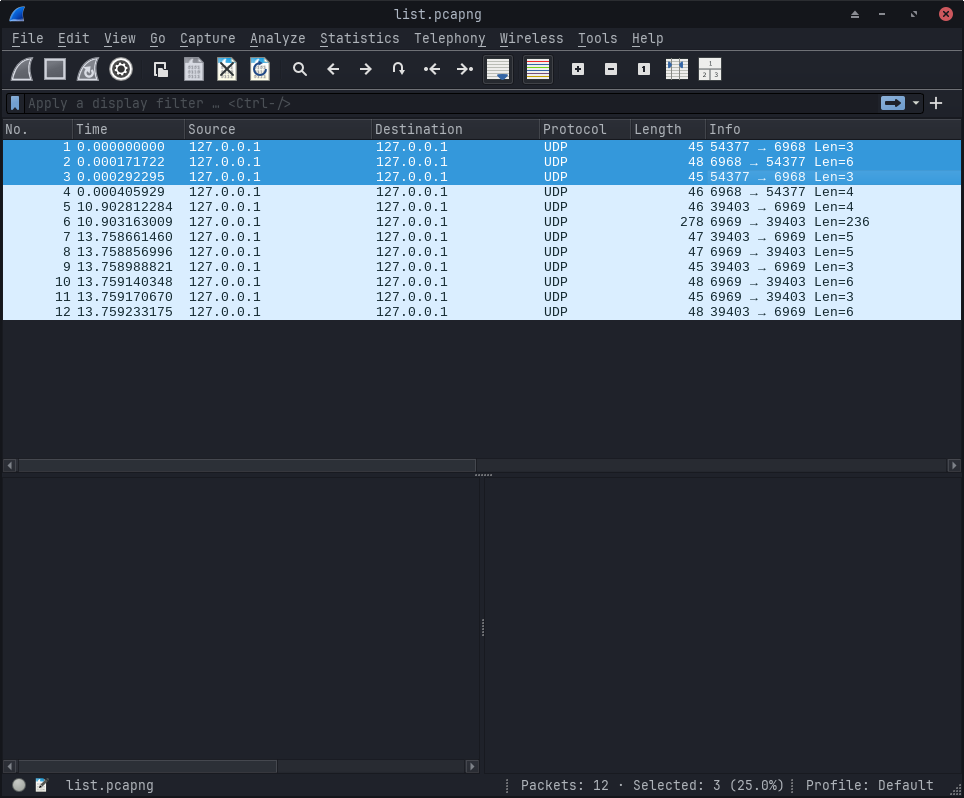
\includegraphics[width=0.6\textwidth]{imgs/03/syn-synack-ack.png}
    \caption{Three-Way Handshake: \lstinlinebg{SYN}, \lstinlinebg{SYN-ACK} e \lstinlinebg{ACK}}
    \label{fig:syn-synack-ack}
\end{figure}

successivamente, dopo che il server si è duplicato (tramite la funzione \lstinlinebg{fork()}) viene inviata la porta \lstinlinebg{6969} dal server al client, come mostrato in Fig. \ref{fig:port-6969}.

\begin{figure}[h]
    \centering
    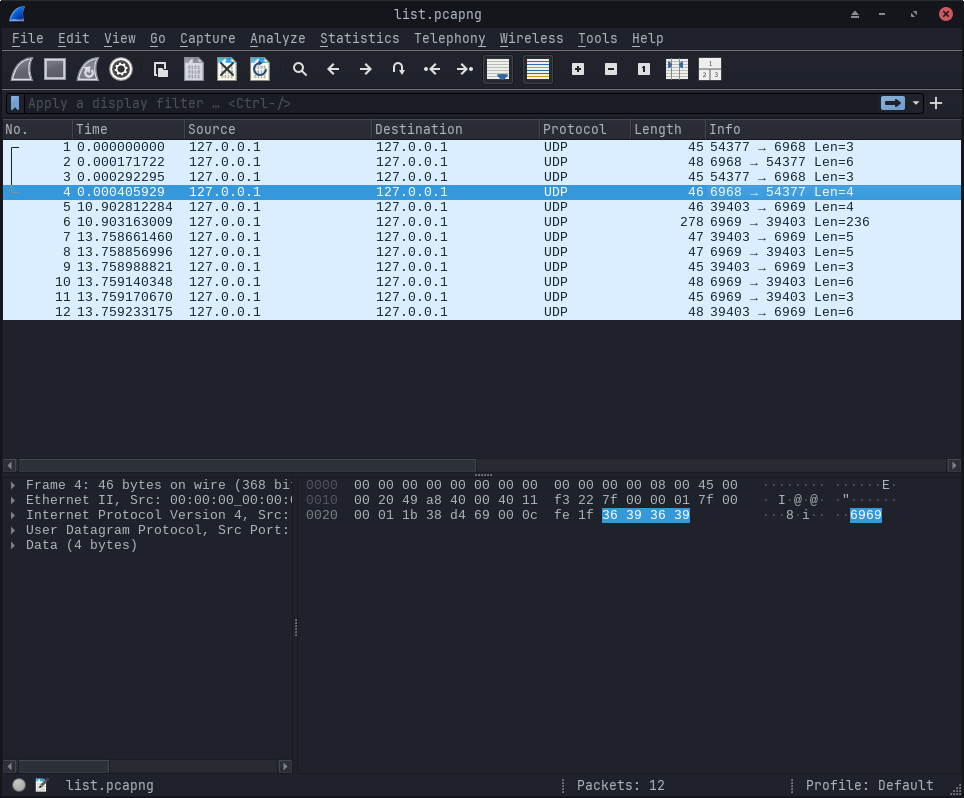
\includegraphics[width=0.6\textwidth]{imgs/03/port.png}
    \caption{Porta \lstinlinebg{6969} inviata dal server al client}
    \label{fig:port-6969}
\end{figure}

Il server risponde con la lista dei file disponibili, come mostrato in Fig. \ref{fig:list}.

\begin{figure}[h]
    \centering
    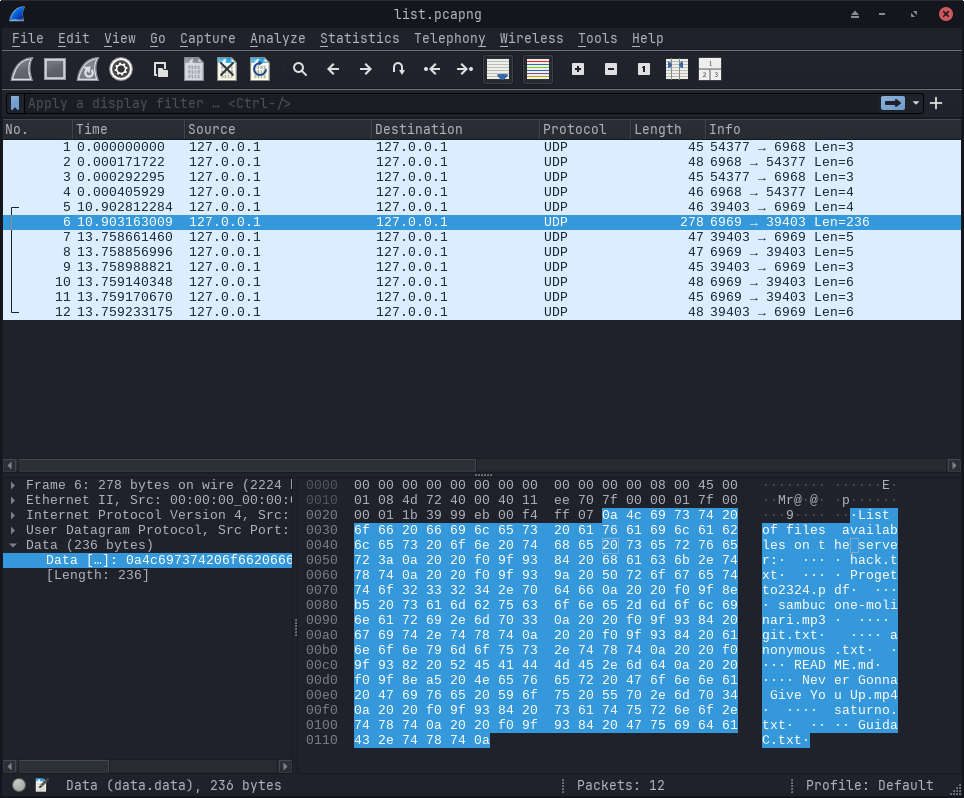
\includegraphics[width=0.6\textwidth]{imgs/03/list-cmd.png}
    \caption{Lista dei file disponibili inviata dal server al client}
    \label{fig:list}
\end{figure}

Infine viene chiusa la connessione tra il client e il server.
In particolare viene usato il comado \lstinlinebg{CLOSE} per chiudere la connessione, tramite i pacchetti \lstinlinebg{FIN}, \lstinlinebg{FIN-ACK}, \lstinlinebg{FIN} e \lstinlinebg{FIN-ACK}, come mostrato in Fig. \ref{fig:fin-finack-ack}.

\begin{figure}[h]
    \centering
    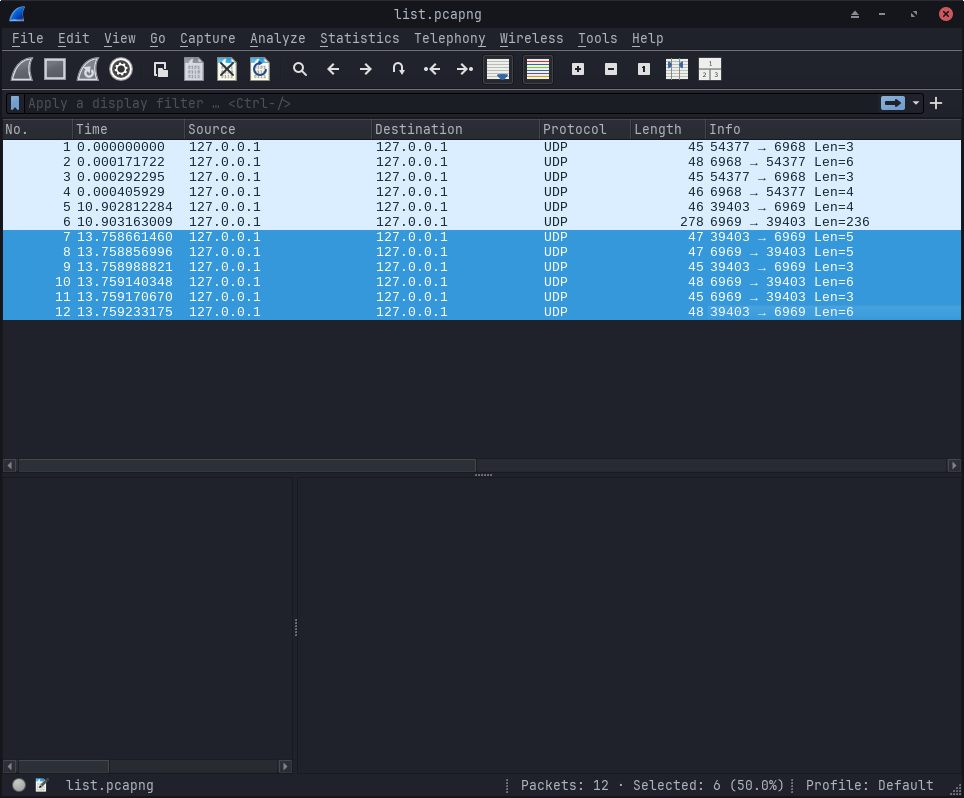
\includegraphics[width=0.6\textwidth]{imgs/03/close-CLOSE-fin-finack-fin-finack.png}
    \caption{Three-Way Handshake: \lstinlinebg{CLOSE}, \lstinlinebg{FIN}, \lstinlinebg{FIN-ACK}, \lstinlinebg{FIN} e \lstinlinebg{FIN-ACK}}
    \label{fig:fin-finack-ack}
\end{figure}

\subsection{Esempio d'uso del comando \lstinlinebig{GET}}
Utilizzando il comando \lstinlinebg{GET} è possibile effettuare il download di un file dal server.
Per usare tale comando è richiesto l'utilizzo del comando \lstinlinebg{LIST} per ottenere la lista dei file disponibili sul server per scegliere il file da scaricare.
Nel caso in cui il file non sia presente sul server, viene stampato il seguente messaggio:

\begin{lstlisting}[numbers=none,escapeinside={(*}{*)}]
(*\emoji{red-question-mark}*) Filename not found.
\end{lstlisting}

\subsubsection{Esempio con probabilità di perdita del 20\%}
Se il file richiesto è presente nella directory \lstinlinebg{server-files/} e la probabilità di perdita dei pacchetti è del 20\%, il file viene scaricato con successo:

\begin{lstlisting}[numbers=none,escapeinside={(*}{*)}]
[client@spqr ~]$ get

(*\emoji{open-file-folder}*) Insert file to transfer: GuidaC.txt

[100.0%] [(*\emoji{package}*)(*\emoji{package}*)(*\emoji{package}*)(*\emoji{package}*)(*\emoji{package}*)(*\emoji{package}*)(*\emoji{package}*)(*\emoji{package}*)(*\emoji{package}*)(*\emoji{package}*)(*\emoji{package}*)(*\emoji{package}*)(*\emoji{package}*)(*\emoji{package}*)(*\emoji{package}*)(*\emoji{package}*)(*\emoji{package}*)(*\emoji{package}*)(*\emoji{package}*)(*\emoji{package}*)]

    ╔═════════════════════════════════╗
    ║ FILE TRANSFER COMPLETED         ║
    ╠═════════════════════════════════╣
    ║ TIME       = 2.429695 sec       ║
    ║ THROUGHPUT = 825.52 KB/s        ║
    ╚═════════════════════════════════╝    
\end{lstlisting}

\subsubsection{Esempio con probabilità di perdita dell'80\%}
Se il file richiesto è presente nella directory \lstinlinebg{server-files/} e la probabilità di perdita dei pacchetti è dell'80\%, il file non viene scaricato:

\begin{lstlisting}[numbers=none,escapeinside={(*}{*)}]
[client@spqr ~]$ get

(*\emoji{open-file-folder}*) Insert file to transfer: GuidaC.txt

[7.7%] [(*\emoji{package}*)                   ]

    ╔═════════════════════════════════╗
    ║ FILE TRANSFER FAILED            ║
    ╠═════════════════════════════════╣
    ║ TIME       = 18.794660 sec      ║
    ║ THROUGHPUT = 8.18 KB/s          ║
    ╚═════════════════════════════════╝    
\end{lstlisting}


\subsection{Esempio d'uso del comando \lstinlinebig{PUT}}
Utilizzando il comando \lstinlinebg{PUT} è possibile effettuare l'upload di un file sul server.
Nel caso in cui il file non sia presente sul client, viene stampato il seguente messaggio:

\begin{lstlisting}[numbers=none,escapeinside={(*}{*)}]
(*\emoji{red-question-mark}*) File "<filename>" not found.
\end{lstlisting}

Mentre se il file è già presente sul server, viene stampato il seguente messaggio:

\begin{lstlisting}[numbers=none,escapeinside={(*}{*)}]
(*\emoji{open-file-folder}*) File exists on the server.
\end{lstlisting}

\subsubsection{Esempio con probabilità di perdita del 20\%}
Se il file richiesto è presente nella directory \lstinlinebg{client-files/} e la probabilità di perdita dei pacchetti è del 20\%, il file viene caricato con successo:

\begin{lstlisting}[numbers=none,escapeinside={(*}{*)}]
[client@spqr ~]$ put

List of files in the client-files/ directory:
  (*\emoji{page-facing-up}*) GuidaC.txt
    
(*\emoji{open-file-folder}*) Insert file to transfer: GuidaC.txt

[100.0%] [(*\emoji{package}*)(*\emoji{package}*)(*\emoji{package}*)(*\emoji{package}*)(*\emoji{package}*)(*\emoji{package}*)(*\emoji{package}*)(*\emoji{package}*)(*\emoji{package}*)(*\emoji{package}*)(*\emoji{package}*)(*\emoji{package}*)(*\emoji{package}*)(*\emoji{package}*)(*\emoji{package}*)(*\emoji{package}*)(*\emoji{package}*)(*\emoji{package}*)(*\emoji{package}*)(*\emoji{package}*)]

    ╔═════════════════════════════════╗
    ║ FILE TRANSFER COMPLETED         ║
    ╠═════════════════════════════════╣
    ║ TIME       = 2.149967 sec       ║
    ║ THROUGHPUT = 932.93 KB/s        ║
    ╚═════════════════════════════════╝   
\end{lstlisting}

\subsubsection{Esempio con probabilità di perdita dell'80\%}
Se il file richiesto è presente nella directory \lstinlinebg{client-files/} e la probabilità di perdita dei pacchetti è dell'80\%, il file non viene caricato:

\begin{lstlisting}[numbers=none,escapeinside={(*}{*)}]
[client@spqr ~]$ put

List of files in the client-files/ directory:
  (*\emoji{page-facing-up}*) GuidaC.txt

(*\emoji{open-file-folder}*) Insert file to transfer: GuidaC.txt

[6.1%] [(*\emoji{package}*)                   ]

    ╔═════════════════════════════════╗
    ║ FILE TRANSFER FAILED            ║
    ╠═════════════════════════════════╣
    ║ TIME       = 17.066263 sec      ║
    ║ THROUGHPUT = 117.53 KB/s        ║
    ╚═════════════════════════════════╝
\end{lstlisting}

\subsection{Esempio d'uso del comando \lstinlinebig{CLOSE}}
Per chiudere la connessione tra il server e il client è possibile utilizzare il comando \lstinlinebg{CLOSE}.
In particolare, il client viene terminato correttamente con il seguente messaggio:

\begin{lstlisting}[numbers=none,escapeinside={(*}{*)}]
[client@spqr ~]$ close

Bye bye! (*\emoji{wave}*)
\end{lstlisting}

mentre il server rimane in attesa di connessioni da parte di altri client, annotando nella memoria condivisa che si è liberata una posizione, utilizzando il seguente messaggio:

\begin{lstlisting}[numbers=none]
Closed connection for client #0 on port 6969 with exit code 0.
\end{lstlisting}

\subsubsection{Chiusura del server e del client con \lstinlinebig{ctrl+c}}
Inoltre è possibile chiudere il server e il client utilizzando la combinazione \lstinlinebg{ctrl+c} (corrispondente al segnale \lstinlinebg{SIGINT}) sulla tastiera.
In particolare, se il client viene chiuso con \lstinlinebg{ctrl+c}, si ottiene il seguente messaggio:

\begin{lstlisting}[numbers=none,escapeinside={(*}{*)}]
[client@spqr ~]$ close

Bye bye! (*\emoji{wave}*)
\end{lstlisting}

e il server stampa il seguente messaggio:

\begin{lstlisting}[numbers=none]
Closed connection for client #0 on port 6969 with exit code 0.
\end{lstlisting}

Viceversa, se il server viene chiuso con \lstinlinebg{ctrl+c}, esso comunica a tutti i client connessi che la connessione è stata chiusa, quindi solo nel momento in cui un client tenta di comunicare con il server (inviando un comando) si ottiene il seguente messaggio:

\begin{lstlisting}[numbers=none,escapeinside={(*}{*)}]
[client@spqr ~]$ list
(*\emoji{stop-sign}*) Session terminated by server.

Bye bye! (*\emoji{wave}*)
\end{lstlisting}

Quando tutti i client si sono disconnessi, il server si chiude correttamente con il seguente messaggio:

\begin{lstlisting}[numbers=none,escapeinside={(*}{*)}]
Bye bye! (*\emoji{wave}*)
\end{lstlisting}

\chapter{Valutazione delle prestazioni \emoji{bar-chart}}

In questo capitolo verranno descritti i test effettuati per valutare le prestazioni del sistema.
In modo particolare, verranno analizzati i tempi di trasferimento di un file di dimensione fissa, tra due host connessi sulla stessa rete, al variare di alcune configurazioni del sistema.
Infine verranno presentati i risultati ottenuti e le considerazioni finali.

\section{Ambiente di test}
Nonostante il software S.P.Q.R. sia \textit{cross-platform (Unix-based)}, i test delle performance che sono illustrati in questo capitolo sono stati effettuati su un ThinkPad T480 con le seguenti specifiche:

\begin{itemize}
    \item Processore Intel Core i7-8550U
    \item 32GB di RAM DDR4
    \item Sistema Operativo Linux Manjaro \lstinlinebg{v25.0.0}
\end{itemize}

\subsection{Ambiente Linux}
Il software è stato sviluppato e testato utilizzando i seguenti strumenti:

\begin{itemize}
    \item \lstinlinebg{clang v19.1.7}
    \item Valgrind \lstinlinebg{v3.24.0}
    \item Visual Studio Code \lstinlinebg{v1.97.2}
    \item Wireshark \lstinlinebg{v4.4.3}
\end{itemize}

dove \lstinlinebg{clang} è stato utilizzato come compilatore, \lstinlinebg{valgrind} per il controllo dei memory leak e Visual Studio Code come ambiente di sviluppo.

\subsection{Ambiente MacOS ARM e Intel}
Inoltre il software è stato testato su un MacBook Air del 2020 con le seguenti specifiche:

\begin{itemize}
    \item Processore Apple M1
    \item 8GB di RAM DDR4
    \item MacOS Sequoia
\end{itemize}

e su un MacBook Pro del 2015 con le seguenti specifiche:

\begin{itemize}
    \item Processore Intel Core i5
    \item 16GB di RAM
    \item MacOS Monterey
\end{itemize}

dove per entrambi si è utilizzata l'ultima versione disponibile del compilatore \lstinlinebg{clang}, ovvero la versione \lstinlinebg{v16.0.0}.
Infine si è scelto di non includere i risultati dei test svolti in ambiente Apple, in quanto risultano essere simili a quelli ottenuti su Linux e quindi non fornirebbero alcun valore aggiunto.

\section{Test effettuati}
Per valutare le prestazioni del sistema sono stati effettuati diversi test di trasferimento utilizzando il file di testo chiamato \lstinlinebg{GuidaC.txt} avente dimensione fissa pari a 2.1MB.

\subsection{Test Timeout Adattivo}
Durante l'esecuzione di questo test sono stati utilizzati dei valori della probabilità di perdita nell'intervallo $[0\%, 80\%]$, una dimensione della finestra nell'intervallo $[8, 128]$ e un timeout adattivo impostato nel range $[8000 \mu s, 80000 \mu s]$.
Mettendo insieme tutti i risultati ottenuti dai test è stato possibile costruire la seguente tabella:

\begin{table}[htbp]
    \centering
    \renewcommand{\arraystretch}{1.3} % Aumenta spaziatura verticale
    \caption{Throughput in funzione della finestra e della probabilità di perdita.}
    \label{tab:throughput_adaptive}
    \begin{tabular}{
        >{\centering\arraybackslash}p{1.5cm}|
        >{\centering\arraybackslash}p{2.2cm}|
        >{\centering\arraybackslash}p{1.75cm}|
        >{\centering\arraybackslash}p{1.75cm}|
        >{\centering\arraybackslash}p{1.75cm}|
        >{\centering\arraybackslash}p{1.75cm}|
        >{\centering\arraybackslash}p{1.75cm}
    }
    \toprule
    \rowcolor{headercolor}
    \multicolumn{2}{c|}{\textbf{Timeout Adattivo:}} & \multicolumn{5}{c}{\textbf{Dimensione della Finestra}} \\
    \rowcolor{headercolor}
    \multicolumn{2}{c|}{\textbf{8000 $\boldsymbol{\mu}$s -- 80000 $\boldsymbol{\mu}$s}} & \textbf{8} & \textbf{16} & \textbf{32} & \textbf{64} & \textbf{128} \\
    \midrule
    
    \multirow{10}{*}{\rotatebox[origin=c]{90}{\textbf{Probabilità di Perdita}}} & 
    \cellcolor{rowcolor1}\textbf{0\%} & 
    \cellcolor{rowcolor1}34625.34 & 
    \cellcolor{rowcolor1}35602.67 & 
    \cellcolor{rowcolor1}34971.78 & 
    \cellcolor{rowcolor1}32822.13 & 
    \cellcolor{rowcolor1}16168.72 \\
    
    & \cellcolor{rowcolor2}\textbf{5\%} & 
    \cellcolor{rowcolor2}1670.61 & 
    \cellcolor{rowcolor2}2394.67 & 
    \cellcolor{rowcolor2}3653.44 & 
    \cellcolor{rowcolor2}6061.48 & 
    \cellcolor{rowcolor2}7704.30 \\
    
    & \cellcolor{rowcolor1}\textbf{10\%} & 
    \cellcolor{rowcolor1}965.88 & 
    \cellcolor{rowcolor1}1546.64 & 
    \cellcolor{rowcolor1}2318.92 & 
    \cellcolor{rowcolor1}3808.67 & 
    \cellcolor{rowcolor1}5816.49 \\
    
    & \cellcolor{rowcolor2}\textbf{15\%} & 
    \cellcolor{rowcolor2}695.77 & 
    \cellcolor{rowcolor2}1078.24 & 
    \cellcolor{rowcolor2}1831.08 & 
    \cellcolor{rowcolor2}2836.82 & 
    \cellcolor{rowcolor2}4606.03 \\
    
    & \cellcolor{rowcolor1}\textbf{20\%} & 
    \cellcolor{rowcolor1}521.22 & 
    \cellcolor{rowcolor1}827.01 & 
    \cellcolor{rowcolor1}1404.64 & 
    \cellcolor{rowcolor1}2348.13 & 
    \cellcolor{rowcolor1}3766.66 \\
    
    & \cellcolor{rowcolor2}\textbf{25\%} & 
    \cellcolor{rowcolor2}373.66 & 
    \cellcolor{rowcolor2}622.92 & 
    \cellcolor{rowcolor2}993.31 & 
    \cellcolor{rowcolor2}1827.67 & 
    \cellcolor{rowcolor2}2970.95 \\
    
    & \cellcolor{rowcolor1}\textbf{30\%} & 
    \cellcolor{rowcolor1}312.59 & 
    \cellcolor{rowcolor1}500.43 & 
    \cellcolor{rowcolor1}842.40 & 
    \cellcolor{rowcolor1}1495.68 & 
    \cellcolor{rowcolor1}2421.00 \\
    
    & \cellcolor{rowcolor2}\textbf{40\%} & 
    \cellcolor{rowcolor2}187.29 & 
    \cellcolor{rowcolor2}339.71 & 
    \cellcolor{rowcolor2}518.07 & 
    \cellcolor{rowcolor2}1037.10 & 
    \cellcolor{rowcolor2}1778.96 \\
    
    & \cellcolor{rowcolor1}\textbf{60\%} & 
    \cellcolor{rowcolor1}12.99 & 
    \cellcolor{rowcolor1}41.44 & 
    \cellcolor{rowcolor1}135.48 & 
    \cellcolor{rowcolor1}312.31 & 
    \cellcolor{rowcolor1}589.83 \\
    
    & \cellcolor{rowcolor2}\textbf{80\%} & 
    \cellcolor{rowcolor2}2.88 & 
    \cellcolor{rowcolor2}4.59 & 
    \cellcolor{rowcolor2}7.49 & 
    \cellcolor{rowcolor2}17.72 & 
    \cellcolor{rowcolor2}54.92 \\
    \bottomrule
    \multicolumn{7}{r}{Valori espressi in kB/s} \\
    \end{tabular}
\end{table}

Successivamente, grazie ad uno script automatizzato in Python, è stato possibile costruire il grafico mostrato in Fig. \ref{fig:throughput_adaptive}.

\begin{figure}[htbp]
    \centering
    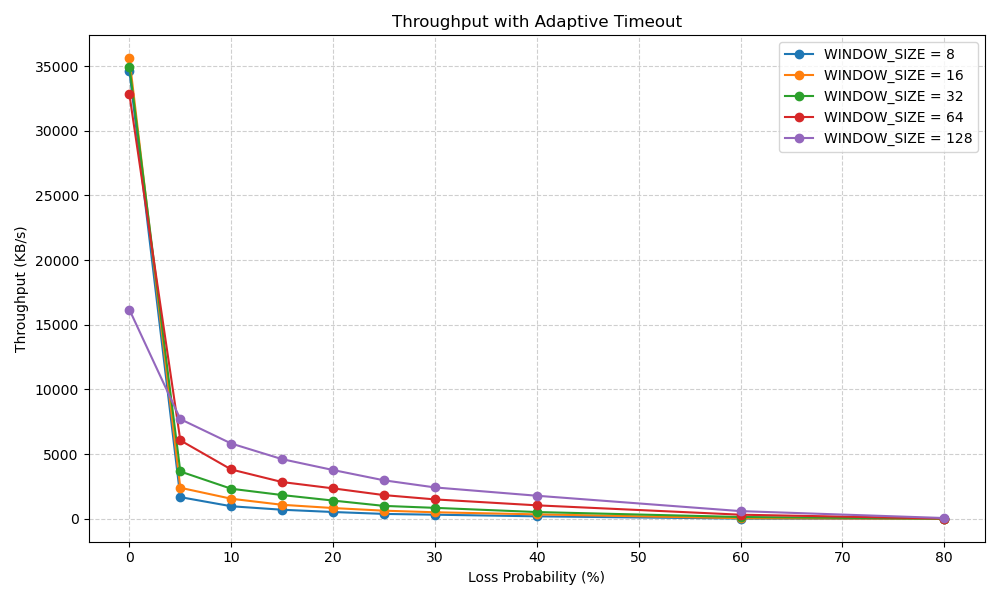
\includegraphics[width=0.65\textwidth]{imgs/04/adaptive-timeout-performance.png}
    \caption{Throughput in funzione della finestra e della probabilità di perdita.}
    \label{fig:throughput_adaptive}
\end{figure}

\subsection{Test Timeout Statico}
Durante l'esecuzione di questo test sono stati utilizzati dei valori della probabilità di perdita nell'intervallo $[0\%, 90\%]$, una dimensione della finestra \lstinlinebg{WINDOW_SIZE} fissa a \lstinlinebg{32} e un timeout statico impostato nel range $[4000 \mu s, 80000 \mu s]$.
Mettendo insieme tutti i risultati ottenuti dai test è stato possibile costruire la seguente tabella:

\begin{table}[htbp]
    \centering
    \renewcommand{\arraystretch}{1.3} % Aumenta spaziatura verticale
    \caption{Throughput in funzione del timeout statico e della probabilità di perdita.}
    \label{tab:throughput_static}
    \begin{tabular}{
        >{\centering\arraybackslash}p{1.2cm}|
        >{\centering\arraybackslash}p{1.5cm}|
        >{\centering\arraybackslash}p{1.6cm}|
        >{\centering\arraybackslash}p{1.6cm}|
        >{\centering\arraybackslash}p{1.6cm}|
        >{\centering\arraybackslash}p{1.6cm}|
        >{\centering\arraybackslash}p{1.6cm}|
        >{\centering\arraybackslash}p{1.6cm}
    }
    \toprule
    \rowcolor{headercolor}
    \multicolumn{2}{c|}{\textbf{Dim. finestra}} & \multicolumn{6}{c}{\textbf{Timeout Statico (in $\boldsymbol{\mu}$s)}} \\
    \rowcolor{headercolor}
    \multicolumn{2}{c|}{\textbf{pari a \textbf{32}}} & \textbf{4000} & \textbf{8000} & \textbf{16000} & \textbf{32000} & \textbf{64000} & \textbf{80000} \\
    \midrule
    
    \multirow{11}{*}{\rotatebox[origin=c]{90}{\textbf{Probabilità di Perdita}}} & 
    \cellcolor{rowcolor1}\textbf{0\%} & 
    \cellcolor{rowcolor1}39653.63 & 
    \cellcolor{rowcolor1}32443.26 & 
    \cellcolor{rowcolor1}28928.45 & 
    \cellcolor{rowcolor1}34412.50 & 
    \cellcolor{rowcolor1}42966.73 & 
    \cellcolor{rowcolor1}36106.52 \\
    
    & \cellcolor{rowcolor2}\textbf{5\%} & 
    \cellcolor{rowcolor2}4727.65 & 
    \cellcolor{rowcolor2}3576.49 & 
    \cellcolor{rowcolor2}2490.50 & 
    \cellcolor{rowcolor2}1277.62 & 
    \cellcolor{rowcolor2}835.57 & 
    \cellcolor{rowcolor2}685.13 \\
    
    & \cellcolor{rowcolor1}\textbf{10\%} & 
    \cellcolor{rowcolor1}3500.83 & 
    \cellcolor{rowcolor1}2502.25 & 
    \cellcolor{rowcolor1}1768.88 & 
    \cellcolor{rowcolor1}909.38 & 
    \cellcolor{rowcolor1}525.79 & 
    \cellcolor{rowcolor1}425.64 \\
    
    & \cellcolor{rowcolor2}\textbf{15\%} & 
    \cellcolor{rowcolor2}2714.11 & 
    \cellcolor{rowcolor2}1914.10 & 
    \cellcolor{rowcolor2}1191.13 & 
    \cellcolor{rowcolor2}655.45 & 
    \cellcolor{rowcolor2}348.69 & 
    \cellcolor{rowcolor2}283.20 \\
    
    & \cellcolor{rowcolor1}\textbf{20\%} & 
    \cellcolor{rowcolor1}2206.86 & 
    \cellcolor{rowcolor1}1512.28 & 
    \cellcolor{rowcolor1}892.03 & 
    \cellcolor{rowcolor1}585.37 & 
    \cellcolor{rowcolor1}267.25 & 
    \cellcolor{rowcolor1}254.48 \\
    
    & \cellcolor{rowcolor2}\textbf{25\%} & 
    \cellcolor{rowcolor2}1694.11 & 
    \cellcolor{rowcolor2}1068.69 & 
    \cellcolor{rowcolor2}690.16 & 
    \cellcolor{rowcolor2}382.73 & 
    \cellcolor{rowcolor2}218.91 & 
    \cellcolor{rowcolor2}164.52 \\
    
    & \cellcolor{rowcolor1}\textbf{30\%} & 
    \cellcolor{rowcolor1}1304.02 & 
    \cellcolor{rowcolor1}926.47 & 
    \cellcolor{rowcolor1}562.95 & 
    \cellcolor{rowcolor1}309.86 & 
    \cellcolor{rowcolor1}170.61 & 
    \cellcolor{rowcolor1}132.60 \\
    
    & \cellcolor{rowcolor2}\textbf{40\%} & 
    \cellcolor{rowcolor2}830.81 & 
    \cellcolor{rowcolor2}578.49 & 
    \cellcolor{rowcolor2}355.41 & 
    \cellcolor{rowcolor2}204.92 & 
    \cellcolor{rowcolor2}108.62 & 
    \cellcolor{rowcolor2}88.31 \\
    
    & \cellcolor{rowcolor1}\textbf{60\%} & 
    \cellcolor{rowcolor1}324.29 & 
    \cellcolor{rowcolor1}221.31 & 
    \cellcolor{rowcolor1}133.52 & 
    \cellcolor{rowcolor1}75.07 & 
    \cellcolor{rowcolor1}39.99 & 
    \cellcolor{rowcolor1}32.43 \\
    
    & \cellcolor{rowcolor2}\textbf{80\%} & 
    \cellcolor{rowcolor2}75.57 & 
    \cellcolor{rowcolor2}50.82 & 
    \cellcolor{rowcolor2}30.73 & 
    \cellcolor{rowcolor2}17.16 & 
    \cellcolor{rowcolor2}9.09 & 
    \cellcolor{rowcolor2}7.36 \\
    
    & \cellcolor{rowcolor1}\textbf{90\%} & 
    \cellcolor{rowcolor1}18.94 & 
    \cellcolor{rowcolor1}12.70 & 
    \cellcolor{rowcolor1}7.62 & 
    \cellcolor{rowcolor1}4.25 & 
    \cellcolor{rowcolor1}2.25 & 
    \cellcolor{rowcolor1}1.35 \\
    \bottomrule
    \multicolumn{8}{r}{Valori espressi in kB/s} \\
    \end{tabular}
\end{table}

Successivamente, grazie ad uno script automatizzato in Python, è stato possibile costruire il grafico mostrato in Fig. \ref{fig:throughput_static}.

\begin{figure}[htbp]
    \centering
    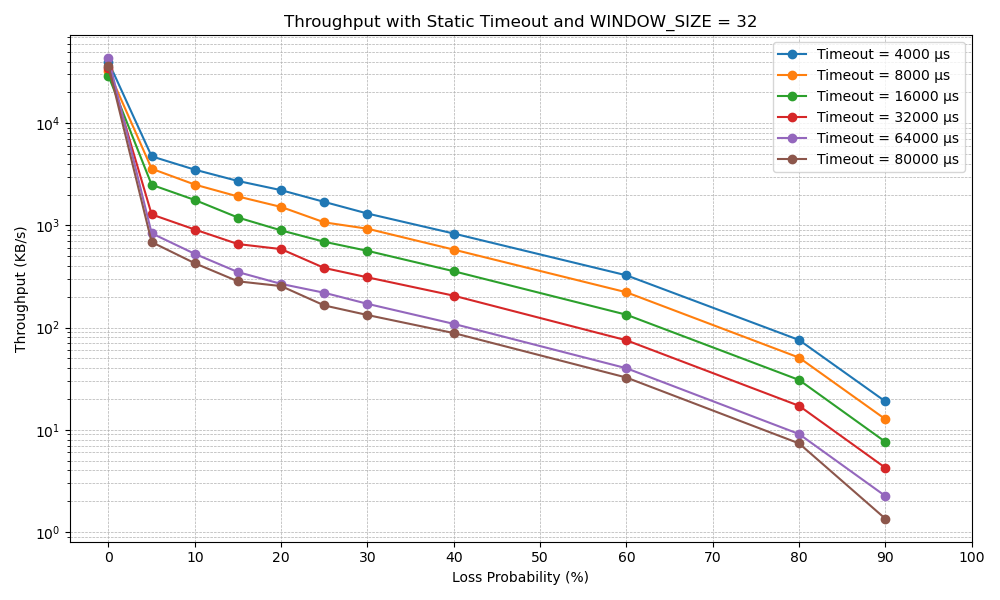
\includegraphics[width=0.65\textwidth]{imgs/04/static-timeout-performance.png}
    \caption{Throughput in funzione del timeout statico e della probabilità di perdita.}
    \label{fig:throughput_static}
\end{figure}

\subsection{Test Timeout Statico \emoji{vs-button} Timeout Adattivo}
Durante l'esecuzione di questo test sono stati riutilizzati i precedenti valori calcolati per il timeout statico e il timeout adattivo e sono stati messi a confronto.
Inoltre è stata aggiunta una colonna relativa alla comulazione di errore per quanto riguarda il timeout adattivo.
Mettendo insieme tutti i risultati ottenuti dai test è stato possibile costruire la seguente tabella:

\begin{table}[htbp]
    \centering
    \renewcommand{\arraystretch}{1.3} % Aumenta spaziatura verticale
    \caption{Confronto throughput fra timeout statico e timeout adattivo.}
    \label{tab:throughput_comparison}
    \begin{tabular}{
        >{\centering\arraybackslash}p{1cm}|
        >{\centering\arraybackslash}p{1.7cm}|
        >{\centering\arraybackslash}p{2.7cm}|
        >{\centering\arraybackslash}p{2cm}|
        >{\centering\arraybackslash}p{1.8cm}|
        >{\centering\arraybackslash}p{1.8cm}|
        >{\centering\arraybackslash}p{1.8cm}
    }
    \toprule
    \rowcolor{headercolor}
    \multicolumn{2}{c|}{\textbf{Dim. finestra}} & 
    \textbf{Cumulazione} & 
    \textbf{Timeout} & 
    \multicolumn{3}{c}{\textbf{Timeout Statici (in $\boldsymbol{\mu}$s)}} \\
    \rowcolor{headercolor}
    \multicolumn{2}{c|}{\textbf{pari a 32}} & \textbf{Errori} & \textbf{Adattivo} & 
    \textbf{8000} & 
    \textbf{32000} & 
    \textbf{80000} \\
    \midrule
    
    \multirow{10}{*}{\rotatebox[origin=c]{90}{\textbf{Probabilità di Perdita}}} &
    \cellcolor{rowcolor1}\textbf{0\%} &
    \cellcolor{rowcolor1}0 &
    \cellcolor{rowcolor1}34971.78 &
    \cellcolor{rowcolor1}32443.26 &
    \cellcolor{rowcolor1}34412.50 &
    \cellcolor{rowcolor1}36106.52 \\
    
    & \cellcolor{rowcolor2}\textbf{5\%} &
    \cellcolor{rowcolor2}34 -- 45 &
    \cellcolor{rowcolor2}3653.44 &
    \cellcolor{rowcolor2}3576.49 &
    \cellcolor{rowcolor2}1277.62 &
    \cellcolor{rowcolor2}685.13 \\
    
    & \cellcolor{rowcolor1}\textbf{10\%} &
    \cellcolor{rowcolor1}53 -- 62 &
    \cellcolor{rowcolor1}2318.92 &
    \cellcolor{rowcolor1}2502.25 &
    \cellcolor{rowcolor1}909.38 &
    \cellcolor{rowcolor1}425.64 \\
    
    & \cellcolor{rowcolor2}\textbf{15\%} &
    \cellcolor{rowcolor2}73 -- 88 &
    \cellcolor{rowcolor2}1831.08 &
    \cellcolor{rowcolor2}1914.10 &
    \cellcolor{rowcolor2}655.45 &
    \cellcolor{rowcolor2}283.20 \\
    
    & \cellcolor{rowcolor1}\textbf{20\%} &
    \cellcolor{rowcolor1}89 -- 108 &
    \cellcolor{rowcolor1}1404.64 &
    \cellcolor{rowcolor1}1512.28 &
    \cellcolor{rowcolor1}585.37 &
    \cellcolor{rowcolor1}254.48 \\
    
    & \cellcolor{rowcolor2}\textbf{25\%} &
    \cellcolor{rowcolor2}128 -- 138 &
    \cellcolor{rowcolor2}993.31 &
    \cellcolor{rowcolor2}1068.69 &
    \cellcolor{rowcolor2}382.73 &
    \cellcolor{rowcolor2}164.52 \\
    
    & \cellcolor{rowcolor1}\textbf{30\%} &
    \cellcolor{rowcolor1}164 -- 181 &
    \cellcolor{rowcolor1}842.40 &
    \cellcolor{rowcolor1}926.47 &
    \cellcolor{rowcolor1}309.86 &
    \cellcolor{rowcolor1}132.60 \\
    
    & \cellcolor{rowcolor2}\textbf{40\%} &
    \cellcolor{rowcolor2}257 -- 280 &
    \cellcolor{rowcolor2}518.07 &
    \cellcolor{rowcolor2}578.49 &
    \cellcolor{rowcolor2}204.92 &
    \cellcolor{rowcolor2}88.31 \\
    
    & \cellcolor{rowcolor1}\textbf{60\%} &
    \cellcolor{rowcolor1}693 -- 715 &
    \cellcolor{rowcolor1}135.48 &
    \cellcolor{rowcolor1}221.31 &
    \cellcolor{rowcolor1}75.07 &
    \cellcolor{rowcolor1}32.43 \\
    
    & \cellcolor{rowcolor2}\textbf{80\%} &
    \cellcolor{rowcolor2}2980 -- 3082 &
    \cellcolor{rowcolor2}7.49 &
    \cellcolor{rowcolor2}50.82 &
    \cellcolor{rowcolor2}17.16 &
    \cellcolor{rowcolor2}7.36 \\
    \bottomrule
    \multicolumn{7}{r}{Valori espressi in kB/s} \\
    \end{tabular}
\end{table}

Successivamente, grazie ad uno script automatizzato in Python, è stato possibile costruire il grafico mostrato in Fig. \ref{fig:throughput_adaptive_vs_static}.

\begin{figure}[htbp]
    \centering
    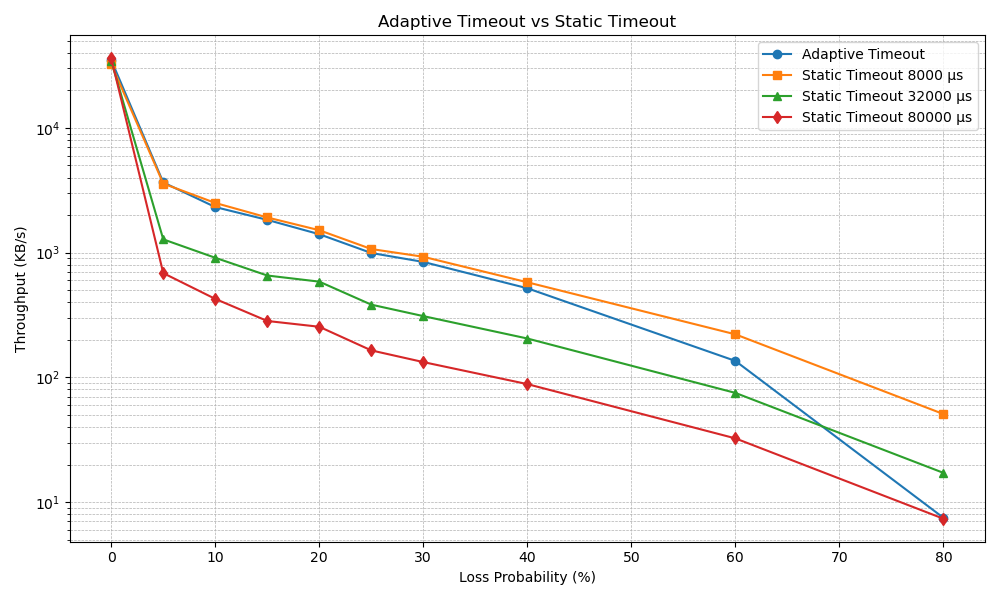
\includegraphics[width=0.65\textwidth]{imgs/04/static-vs-adaptive-timeout-performance.png}
    \caption{Confronto throughput fra timeout statico e timeout adattivo.}
    \label{fig:throughput_adaptive_vs_static}
\end{figure}

\subsection{Test cumulazione degli errori}
Per questo test sono stati utilizzati i valori della comulazione di errore calcolati per il timeout statico e il timeout adattivo e sono stati messi a confronto.
Questi errori vengono memorizzati tramite la variabile \lstinlinebg{max_errors} che tiene traccia del numero massimo di errori consecutivi che si possono verificare durante il trasferimento di un file.
Mettendo insieme tutti i risultati ottenuti dai test è stato possibile costruire la seguente tabella:

\begin{table}[htbp]
    \centering
    \renewcommand{\arraystretch}{1.3} % Aumenta spaziatura verticale
    \caption{Comulazione degli errori in funzione della probabilità di perdita.}
    \label{tab:throughput_error}
    \begin{tabular}{
        >{\centering\arraybackslash}p{1cm}|
        >{\centering\arraybackslash}p{1.75cm}|
        >{\centering\arraybackslash}p{1.75cm}|
        >{\centering\arraybackslash}p{1.75cm}|
        >{\centering\arraybackslash}p{1.75cm}|
        >{\centering\arraybackslash}p{1.75cm}|
        >{\centering\arraybackslash}p{1.75cm}
    }
    \toprule
    \rowcolor{headercolor}
    \multicolumn{2}{c|}{\textbf{Comulazione}} & \multicolumn{5}{c}{\textbf{Dimensione della Finestra}} \\
    \rowcolor{headercolor}
    \multicolumn{2}{c|}{\textbf{Errori}} & \textbf{8} & \textbf{16} & \textbf{32} & \textbf{64} & \textbf{128} \\
    \midrule
    
    \multirow{10}{*}{\rotatebox[origin=c]{90}{\textbf{Probabilità di Perdita}}} & 
    \cellcolor{rowcolor1}\textbf{0\%} & 
    \cellcolor{rowcolor1}0 & 
    \cellcolor{rowcolor1}0 & 
    \cellcolor{rowcolor1}0 & 
    \cellcolor{rowcolor1}0 & 
    \cellcolor{rowcolor1}6 \\
    
    & \cellcolor{rowcolor2}\textbf{5\%} & 
    \cellcolor{rowcolor2}85 -- 99 & 
    \cellcolor{rowcolor2}56 -- 67 & 
    \cellcolor{rowcolor2}34 -- 35 & 
    \cellcolor{rowcolor2}24 -- 30 & 
    \cellcolor{rowcolor2}13 -- 20 \\
    
    & \cellcolor{rowcolor1}\textbf{10\%} & 
    \cellcolor{rowcolor1}127 -- 155 & 
    \cellcolor{rowcolor1}86 -- 92 & 
    \cellcolor{rowcolor1}53 -- 62 & 
    \cellcolor{rowcolor1}32 -- 42 & 
    \cellcolor{rowcolor1}23 -- 25 \\
    
    & \cellcolor{rowcolor2}\textbf{15\%} & 
    \cellcolor{rowcolor2}184 -- 209 & 
    \cellcolor{rowcolor2}122 -- 153 & 
    \cellcolor{rowcolor2}73 -- 88 & 
    \cellcolor{rowcolor2}43 -- 51 & 
    \cellcolor{rowcolor2}26 --30 \\
    
    & \cellcolor{rowcolor1}\textbf{20\%} & 
    \cellcolor{rowcolor1}240 -- 279 & 
    \cellcolor{rowcolor1}169 -- 189 & 
    \cellcolor{rowcolor1}89 -- 108 & 
    \cellcolor{rowcolor1}62 -- 69 & 
    \cellcolor{rowcolor1}32 -- 39 \\
    
    & \cellcolor{rowcolor2}\textbf{25\%} & 
    \cellcolor{rowcolor2}331 -- 348 & 
    \cellcolor{rowcolor2}207 -- 222 & 
    \cellcolor{rowcolor2}128 -- 138 & 
    \cellcolor{rowcolor2}74 -- 82 & 
    \cellcolor{rowcolor2}42 -- 48 \\
    
    & \cellcolor{rowcolor1}\textbf{30\%} & 
    \cellcolor{rowcolor1}444 -- 472 & 
    \cellcolor{rowcolor1}285 -- 297 & 
    \cellcolor{rowcolor1}164 -- 181 & 
    \cellcolor{rowcolor1}98 -- 116 & 
    \cellcolor{rowcolor1}55 -- 61 \\
    
    & \cellcolor{rowcolor2}\textbf{40\%} & 
    \cellcolor{rowcolor2}681 -- 742 & 
    \cellcolor{rowcolor2}453 -- 477 & 
    \cellcolor{rowcolor2}257 -- 280 & 
    \cellcolor{rowcolor2}151 -- 163 & 
    \cellcolor{rowcolor2}87 -- 92 \\
    
    & \cellcolor{rowcolor1}\textbf{60\%} & 
    \cellcolor{rowcolor1}1889 -- 1932 & 
    \cellcolor{rowcolor1}1202 -- 1230 & 
    \cellcolor{rowcolor1}693 -- 715 & 
    \cellcolor{rowcolor1}374 -- 421 & 
    \cellcolor{rowcolor1}140 -- 218 \\
    
    & \cellcolor{rowcolor2}\textbf{80\%} & 
    \cellcolor{rowcolor2}7963 -- 8548 & 
    \cellcolor{rowcolor2}5028 -- 5507 & 
    \cellcolor{rowcolor2}2980 -- 3082 & 
    \cellcolor{rowcolor2}1682 -- 1844 & 
    \cellcolor{rowcolor2}899 -- 1150 \\
    \bottomrule
    \end{tabular}
\end{table}

Successivamente, grazie ad uno script automatizzato in Python, è stato possibile costruire i grafici mostrati in Fig. \ref{fig:throughput_error_static} e Fig. \ref{fig:throughput_error_adaptive}, dove per la comulazione degli errori nel caso del timeout adattivo è stata considerata la colonna della Tabella \ref{tab:throughput_comparison}.

\begin{figure}[htbp]
    \centering
    \begin{minipage}{0.49\textwidth}
        \centering
        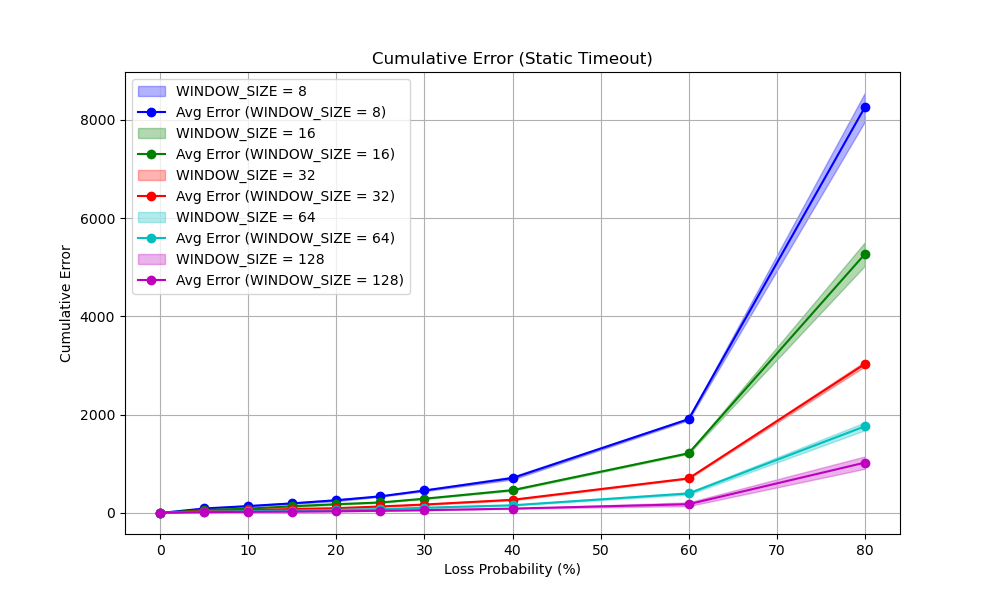
\includegraphics[width=\textwidth]{imgs/04/static-cumulative-error.png}
        \caption{Comulazione degli errori per il timeout statico.}
        \label{fig:throughput_error_static}
    \end{minipage}
    \hfill
    \begin{minipage}{0.49\textwidth}
        \centering
        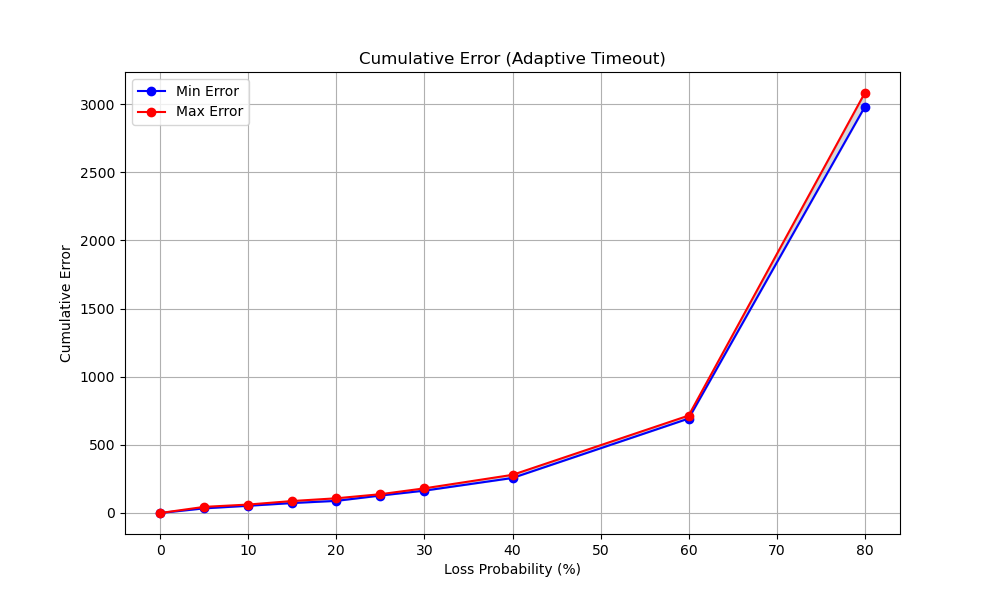
\includegraphics[width=\textwidth]{imgs/04/adaptive-cumulative-error.png}
        \caption{Comulazione degli errori per il timeout adattivo.}
        \label{fig:throughput_error_adaptive}
    \end{minipage}
\end{figure}

\section{Test per l'integrità dei file trasferiti \emoji{snake}}
Infine è stato svolto un test per verificare l'integrità dei file trasferiti.
Per fare ciò è stato creato uno script in Python (presente nella directory \lstinlinebg{tests/}) che confronta il file originale e quello trasferito, verificando che siano identici.
Prima di tutto, il programma calcola l'hash dei file utilizzando un algoritmo di hashing sicuro, come SHA-256, che permette di rilevare rapidamente eventuali differenze nel contenuto.
L'hash viene calcolato leggendo il file a blocchi per ottimizzare l'efficienza anche con file di grandi dimensioni.
Se gli hash di due file sono identici, il programma esegue un ulteriore confronto byte per byte per essere completamente sicuro che i file siano uguali.
Il funzionamento si estende a due directory specificate dall'utente, denominate di default con \lstinlinebg{client-files/} e \lstinlinebg{server-files/}.
Il programma analizza il contenuto di entrambe le directory, confrontando i file con lo stesso nome.
Se due file hanno lo stesso nome ma contenuti differenti, il programma segnala la differenza, evidenziandola in rosso nel terminale.
Se, invece, i file sono uguali, viene indicato un messaggio in verde, confermando che i file sono identici.
Inoltre, il programma elenca anche i file che sono presenti solo in una delle due directory, fornendo un riepilogo completo delle differenze.

\subsection{Esempio di funzionamento}
Per esemplificare il funzionamento dello script, può essere usato il file di testo \lstinlinebg{GuidaC.txt}.
Immaginando che questo file sia stato inviato dal cliente al server (o viceversa).
Per eseguire lo script è sufficiente accedere alla root directory del progetto (ovvero \lstinlinebg{spqr/}) e lanciare il seguente comando:

\begin{lstlisting}[numbers=none]
python tests/integrity-consistency.py
\end{lstlisting}

Un esempio di output dello script è il seguente:

\begin{lstlisting}[numbers=none]
The files "GuidaC.txt" inside "./client-files/" and "./server-files/" are the same.
\end{lstlisting}


\end{document}
